\documentclass[11pt,a4paper]{article}

% ---------------------------------------------------------------------------
% Trustworthy decisions in stochastic amplification assays:
% timing limits, measurement design, and effective capacity.
%
% Author metadata: set the macros below before submission.  They are
% deliberately left blank in this version.
% ---------------------------------------------------------------------------
\newcommand{\PaperAuthor}{}
\newcommand{\PaperAffiliation}{}
\newcommand{\PaperDate}{17 September 2026}
\newcommand{\RepositoryNote}{The repository location will be supplied with the author information.}

\usepackage[T1]{fontenc}
\usepackage[utf8]{inputenc}
\usepackage{lmodern}
\usepackage{microtype}
\usepackage[a4paper,margin=1.05in]{geometry}
\usepackage{amsmath,amssymb,amsthm,mathtools}
\usepackage{booktabs}
\usepackage{array}
\usepackage{enumitem}
\usepackage{xcolor}
\usepackage{graphicx}
\usepackage[obeyspaces,spaces]{url}
\usepackage[numbers,sort&compress]{natbib}
\usepackage[colorlinks=true,linkcolor=blue!55!black,citecolor=blue!55!black,urlcolor=blue!55!black]{hyperref}
\hypersetup{pdftitle={Trustworthy decisions in stochastic amplification assays},
  pdfkeywords={isothermal amplification, digital assays, hypothesis testing, monotone likelihood ratio, pure-birth process, holding times, beta-gamma algebra, identifiability, censoring, formal verification, Lean}}

\DeclareUrlCommand\lean{\urlstyle{tt}}
\setlist{itemsep=2pt,topsep=3pt}
\setlength{\emergencystretch}{1.5em}
\graphicspath{{figures/}}

\theoremstyle{plain}
\newtheorem{theorem}{Theorem}[section]
\newtheorem{proposition}[theorem]{Proposition}
\newtheorem{lemma}[theorem]{Lemma}
\newtheorem{corollary}[theorem]{Corollary}
\theoremstyle{definition}
\newtheorem{definition}[theorem]{Definition}
\theoremstyle{remark}
\newtheorem{remark}[theorem]{Remark}

\newcommand{\R}{\mathbb R}
\newcommand{\N}{\mathbb N}
\newcommand{\E}{\mathbb E}
\newcommand{\Prob}{\mathbb P}
\newcommand{\Var}{\operatorname{Var}}
\newcommand{\FP}{\operatorname{FP}}
\newcommand{\Miss}{\operatorname{Miss}}
\newcommand{\TV}{d_{\mathrm{TV}}}
\newcommand{\Gam}{\operatorname{Gamma}}
\newcommand{\Bet}{\operatorname{Beta}}
\newcommand{\Ex}{\operatorname{Exp}}
\newcommand{\Poi}{\operatorname{Poisson}}
\newcommand{\one}{\mathbf 1}
\newcommand{\dd}{\,\mathrm d}
\newcommand{\eps}{\varepsilon}
\newcommand{\Wc}{\mathcal W}

\title{Trustworthy decisions in stochastic amplification assays:\\
timing limits, measurement design, and effective capacity}
\author{\PaperAuthor\\[2pt]\small\PaperAffiliation}
\date{\PaperDate}

\begin{document}
\maketitle

\begin{abstract}
Changing a readout time, adding an identity-sensitive measurement, increasing the reagent reserve, and improving the inference procedure solve different problems, and a laboratory that confuses them can spend its effort on a step that cannot succeed. We separate these problems for a finite pure-birth amplification source with Poisson loading, a latching detection threshold and an effective resource capacity. For the source at threshold five, every measurable randomized classifier of the complete crossing time that keeps blank error at most $1\%$ misses more than $5.55\%$ of loaded reactions; this all-rule obstruction, its concrete source identities and a source-preserving hit-and-identity repair with blank error below $0.03\%$ and miss below $4.22443\%$ are verified in Lean~4. We then prove, with ordinary mathematics, that for any fixed sequential source with shared kinetics a deadline is optimal among all crossing-time classifiers; this converts every all-deadline exclusion into an all-classifier exclusion and sharpens the certified bound to $6.9\%$. Using the holding-time representation of the crossing time we show that the obstruction is not a small-count artefact: for every integer threshold $h\ge10^{6}$ with the resource exhausted at detection, every crossing-time classifier at $1\%$ blank error misses more than $5.63\%$, an explicit identity measurement misses less than $4.13\%$, and doubling the capacity restores a usable deadline with errors below $0.9373\%$ and $4.8732\%$. The proof replaces earlier Chebyshev allowances by gamma Chernoff and weighted Bernstein bounds and reduces the sufficient threshold from $10^{8}$ to $10^{6}$. For the mechanism question we exhibit two capacities with exactly the same blank endpoint law, prove that calibrated intermediate observations recover capacity through clock-free ordered block ratios with strictly monotone, uniquely invertible ordering probabilities, extend the block theorem to non-exponential factorized holding times, and show that thresholds chosen as fractions of each reaction's own plateau lose the leading capacity information. A signal-to-state interval construction and a censoring-safe confidence procedure that retains every incomplete observation complete an executable analysis. All performance statements are conditional mathematical results; no physical channel, calibration or biochemical resource is asserted to have been measured.
\end{abstract}

\section{Introduction}\label{sec:intro}

A digital amplification reaction can cross its signal threshold because it contained target or because background amplification eventually produced the same product \citep{notomi2000,vogelstein1999,rolando2019,hardinge2019}. An earlier deadline suppresses background at the price of discarding slowly developing target reactions. Four different remedies are routinely discussed: tune the cutoff, add an identity-sensitive readout such as a melt curve \citep{rolando2020}, change the reaction so that more resource remains at detection, or analyse the data more carefully. These are not interchangeable, and the purpose of this paper is to give, for one explicitly declared stochastic source, mathematical diagnostics that tell them apart.

\paragraph{A worked decision.}
Consider a laboratory with a digital assay whose blank wells occasionally cross threshold and whose loaded wells contain on average four target units. The operating limits are a $1\%$ blank error and a $5\%$ miss per reaction. The questions that determine the next experiment are the following.
\begin{enumerate}[label=(\arabic*)]
\item \emph{Is there a readout time at which both limits hold?} If the answer is provably no for every deadline, cutoff tuning is futile. Section~\ref{sec:timing} certifies such an instance.
\item \emph{Could a cleverer rule on the same crossing-time datum do better than a deadline?} For the declared source the answer is no: Theorem~\ref{thm:mlr} shows that the best measurable randomized function of the complete crossing time is a deadline. A negative answer to (1) is therefore an information obstruction, not a search failure.
\item \emph{What would an additional measurement have to achieve?} Proposition~\ref{prop:channel} gives the hit-conditioned sensitivity and false-positive rate that make a hit-and-identity rule meet the limits, and Section~\ref{sec:timing} exhibits a joint observation law realizing them without changing the count kinetics.
\item \emph{Would the conclusion change at realistic thresholds?} Section~\ref{sec:large} shows it does not: at every threshold $h\ge10^{6}$ with the resource exhausted at detection the obstruction persists with explicit constants, while a doubled capacity restores a deadline. Which of these regimes an assay occupies is decided by its remaining headroom at detection, not by the size of the count.
\item \emph{Does a failing timing rule identify the mechanism?} No: Section~\ref{sec:capacity} exhibits two capacities with identical blank endpoint laws, and shows what calibrated intermediate observations do and do not recover.
\item \emph{How should incomplete observations be treated?} Section~\ref{sec:inference} shows that deleting slow reactions reintroduces the very clock dependence the method removes, and gives a confidence procedure that retains every observation and returns an interval, a one-sided bound, an unresolved verdict or a model incompatibility.
\end{enumerate}

\paragraph{Main results in words.}
The source is a pure-birth chain on $\{0,\dots,h\}$ with rate $(b+gz)(1-z/R)$ from count $z$, latched at the threshold $h$, with Poisson loading of mean $\lambda$ (Section~\ref{sec:source}). Writing $a=b/g$, the nominal instance has $a=.01$, $\lambda=4$ and limits $\alpha=.01$, $\beta=.05$.
\begin{enumerate}[label=(\roman*)]
\item At $R=h=5$, every measurable randomized classifier of the complete crossing time with blank error at most $.01$ has miss greater than $.0555$; a source-preserving hit-and-identity rule at model time seven has blank error below $.0003$ and miss below $.0422443$, an advantage of more than $1.32557$ percentage points (Theorem~\ref{thm:separation}; Lean-verified).
\item For any fixed positive pre-hit rates shared by both classes, and any Poisson (indeed any) loading law, a deadline at the blank $\alpha$-quantile maximizes power among all measurable randomized crossing-time classifiers (Theorem~\ref{thm:mlr}; ordinary proof). Combined with the certified separating time at $t=5$ this sharpens (i) to miss greater than $.069$, and combined with exact enclosures at threshold twenty it excludes every classifier there with miss greater than $.087$ (Corollary~\ref{cor:sharp}).
\item Classwise total-variation budgets, a $\pm2\%$ fixed-rate operating window, and a label-neutral-pipeline comparison show what the certified separation tolerates and what cannot repair it (Propositions~\ref{prop:tv}--\ref{prop:pipeline}).
\item The crossing time is a sum of independent exponential holding times whose undepleted part has an exact beta law. With a growing reserve, depletion is a deterministic delay and the limiting tradeoff is the undepleted one; with fixed headroom $m$, the last $m+1$ births add an independent $\Gam(m+1)$ delay in logarithmic time (Theorems~\ref{thm:reserve}--\ref{thm:headroom}). For every integer $h\ge10^{6}$: at $R=h$ every crossing-time classifier at $1\%$ blank error misses more than $5.63\%$, an explicit identity measurement misses less than $4.13\%$ with blank error below $0.085\%$, and at $R=2h$ an explicit deadline has errors below $.009373$ and $.048732$ (Theorem~\ref{thm:big}; ordinary proof with directed scalar certificates).
\item At threshold three the sources $(b,g,R)=(2,1,6)$ and $(8/3,2/3,4)$ have identical blank crossing-time measures (Proposition~\ref{prop:nonident}; Lean-verified). With $a$ known and calibrated states observed, paired waits and ordered block ratios cancel an unknown constant clock and recover capacity; the block ordering probability is strictly decreasing and uniquely invertible on its physical range (Theorems~\ref{thm:blocks}--\ref{thm:strict}), the pathwise ordering survives non-exponential, correlated, factorized holding times (Proposition~\ref{prop:general}), and plateau-relative thresholds converge to a capacity-free limit (Proposition~\ref{prop:plateau}).
\item A signal-to-state interval construction, a censoring-safe confidence theorem that needs no independent-censoring assumption (Theorem~\ref{thm:censor}), and a three-way decision procedure with Lean-verified band logic turn the theory into an executable analysis (Section~\ref{sec:inference}).
\end{enumerate}

\paragraph{Three kinds of evidence.}
Every statement below carries one of the following labels. \emph{Lean-verified} statements are theorems of a frozen Lean~4/Mathlib development \citep{demoura2021,mathlib2020}, compiled with warnings treated as errors and depending only on the standard axioms; Section~\ref{sec:verification} and Appendix~\ref{app:map} list them. \emph{Ordinary proof} means a complete mathematical argument printed here; it has not thereby become a Lean declaration. \emph{Exact rational computation} and \emph{directed computation} mean that integer or rational arithmetic, or outward rounding with explicit remainder bounds, certifies the stated finite inequalities; the script \path{check_paper.py} replays all of them. \emph{Numerical illustration} means a floating-point evaluation, root or seeded simulation; such values are never premises of a theorem. \emph{Empirical} conclusions require physical observations, and none is established here.

\paragraph{Relation to prior work.}
The tradeoff between speed, sensitivity and background is established experimental territory \citep{rolando2019,hardinge2020,hardinge2019,schneider2019}, and kinetic and identity information have already been combined in real-time digital LAMP with high-resolution melting \citep{rolando2020}; adding identity information is therefore not itself the contribution. On the statistical side, optimality of likelihood-ratio tests \citep{neyman1933}, the monotone-likelihood-ratio theory \citep{karlinrubin1956,lehmannromano2005}, comparison of experiments \citep{blackwell1953}, the beta--gamma algebra \citep{lukacs1955}, the logarithmic limit of the Yule process \citep{kendall1948} and the concentration inequalities we use \citep{hoeffding1963,boucheron2013} are classical, and we claim no priority for them. The contribution is their source-connected combination: a concrete, formally checked separation between a timing experiment and an identity experiment; the general deadline-optimality theorem that makes the separation an information statement; an explicit large-threshold theorem showing that neither concentration of large counts nor the vanishing of initial hits removes it; and observation-design results for effective capacity that distinguish exact nonidentification, loss of conditioning, selection bias and normalization artefacts. The certified capacity classification at threshold five that this paper builds on is in a companion manuscript \citep{companion2026}.

\paragraph{What is not claimed.}
The units of the source are effective amplification units, not molecules or fluorescence; rate constants are illustrative; the capacity is an effective inventory whose laboratory realization is an open question; the assumed $99\%/1\%$ channel capabilities are stated premises, not measured performance; and no biological dataset is used to fit or validate any constant. Neither clinical performance nor priority over the experimental literature is asserted. The results do not establish universal necessity of an identity readout: the reserve regime of Section~\ref{sec:large} is a positive control in which timing alone works.

\paragraph{Organization.}
Section~\ref{sec:source} defines the source, the observations and the decision unit. Section~\ref{sec:timing} contains the certified separation, the deadline-optimality theorem and the robustness propositions. Section~\ref{sec:large} contains the large-threshold theory. Section~\ref{sec:capacity} treats effective capacity. Section~\ref{sec:inference} treats signal calibration, incomplete observations and the decision procedure. Section~\ref{sec:discussion} states the scope and the empirical frontier, and Section~\ref{sec:verification} the verification and reproduction record. Appendices~\ref{app:source}--\ref{app:map} contain the source calculation, the sign certificate, the proof of Theorem~\ref{thm:big} with its directed arithmetic, and the claims-to-declarations map.

\section{The source, the observations, and the decision unit}\label{sec:source}

\subsection{Counts, capacity, loading and classifiers}
Let $X_t$ be a continuous-time pure-birth chain on $\{0,\dots,h\}$, latched (absorbed) at $h$, with pre-hit rates
\begin{equation}\label{eq:rate}
q_z=(b+gz)\Bigl(1-\frac zR\Bigr),\qquad 0\le z<h,\quad b,g>0,\quad R>h-1.
\end{equation}
Here $b$ is background initiation, $gz$ is growth proportional to the active count and $1-z/R$ is the resource factor; $R-z$ is the remaining effective inventory. Target-origin and background-origin units grow with the same coefficient, so the total count is a closed observable. The crossing time is $T=\inf\{t:X_t=h\}$. A \emph{blank} starts at zero. A \emph{loaded} preparation starts at $\min(N,h)$, where $N\sim\Poi(\lambda)$ is independent of the subsequent source innovations; loads $N\ge h$ give an atom of $T$ at zero, which is retained. Write
\[
F(t)=\Prob_0(T\le t),\qquad M(t)=\Prob_1(T>t),
\]
for the blank crossing probability and the loaded miss probability of the deadline $t$. Time is model time; a physical rate calibration is needed before a numerical deadline is an assay turnaround time. Writing $a=b/g$ and $\tau=gT$ removes $g$ from every statement.

The decision unit is one reaction, and empty loaded reactions ($N=0$) remain in the denominator. A \emph{measurable randomized complete-time classifier} is a measurable $\phi:[0,\infty)\to[0,1]$, interpreted as the probability of calling a reaction positive when its crossing time is $T$; its errors are
\begin{equation}\label{eq:errors}
\FP(\phi)=\E_0\,\phi(T),\qquad \Miss(\phi)=1-\E_1\,\phi(T).
\end{equation}
A deadline is $\phi(t)=\one\{t\le t_0\}$. Complete timing reveals the eventual crossing time even beyond any finite acquisition, so an obstruction for complete-time classifiers is an obstruction for every finite acquisition of the same datum. The nominal instance is
\begin{equation}\label{eq:nominal}
b=\tfrac1{100},\quad g=1,\quad R=h=5,\quad\lambda=4,\qquad\alpha=\tfrac1{100},\quad\beta=\tfrac1{20}.
\end{equation}
Both classes share the post-loading rates \eqref{eq:rate}. An assay in which target and background products have different subsequent kinetics is a different source: the decision-theoretic method applies, but the constants do not transfer.

\begin{proposition}[Loading floor; ordinary proof]\label{prop:floor}
If an empty loaded reaction has the blank observation law, then every rule with blank error at most $\alpha$ has $\Miss\ge e^{-\lambda}(1-\alpha)$. Miss at most $\beta$ therefore requires $\lambda\ge\log((1-\alpha)/\beta)$, which is $2.9857$ at the nominal limits; at $\lambda=4$ the floor is $.018133$.
\end{proposition}
\begin{proof}
The loaded law is $P_1=e^{-\lambda}P_0+(1-e^{-\lambda})P_{\rm occ}$. Integrate $1-\phi\ge0$ against it and rearrange.
\end{proof}
The floor concerns loaded preparations, not occupancy-conditioned sensitivity. Splitting a fixed specimen among several wells changes the loading, so independence alone does not justify raising a per-reaction miss to a power.

\subsection{The probability law and the holding-time representation}\label{sec:law}
The formal development defines every probability through uniformization \citep{jensen1953,norris1997}: with $\nu\ge\max_zq_z$ and $P=I+Q/\nu$ for the generator $Q$ of the chain, the transition matrix is $K_t=e^{-\nu t}\sum_k(\nu t)^kP^k/k!=e^{tQ}$, and $F$, $M$ are the corresponding Poisson mixtures (Appendix~\ref{app:source}). The conventional arguments use instead the holding-time construction.

\begin{lemma}[Holding times; ordinary proof]\label{lem:holding}
Let $E_n,\dots,E_{h-1}$ be independent unit exponential variables. The crossing time from state $n<h$ satisfies
\begin{equation}\label{eq:holding}
T_n\ \overset{d}{=}\ \sum_{z=n}^{h-1}\frac{E_z}{q_z}
=\frac1g\,\frac{R}{R+a}\Bigl[\sum_{z=n}^{h-1}\frac{E_z}{z+a}+\sum_{z=n}^{h-1}\frac{E_z}{R-z}\Bigr].
\end{equation}
\end{lemma}
\begin{proof}
A pure-birth chain holds in state $z$ for an $\Ex(q_z)$ time and moves to $z+1$; successive holding times are independent by the strong Markov property \citep{feller1968,norris1997}. The transition matrix of this construction solves the finite forward equation $K'_t=K_tQ$, $K_0=I$, whose unique solution is $e^{tQ}$; so it coincides with the uniformized law (Appendix~\ref{app:source}). The second form is partial fractions.
\end{proof}
The first sum in \eqref{eq:holding} is the undepleted crossing time and the second is the resource delay; they share the same $E_z$ and are not independent at finite $h$. The identification of the uniformized law with the holding-time construction is an ordinary finite-state proof; it is not formalized, and no coupling argument below is labeled Lean-verified.

\begin{table}[htbp]\centering\small
\begin{tabular}{>{\raggedright\arraybackslash}p{.28\linewidth}>{\raggedright\arraybackslash}p{.36\linewidth}>{\raggedright\arraybackslash}p{.28\linewidth}}\toprule
Question & Diagnostic supplied & Evidence\\\midrule
Does any readout time work? & Separating-time certificates; usable/excluded/unresolved bands (Section~\ref{sec:procedure}) & Lean at $h=5$, $R=5$ and $10$; exact computation at $h=20$; ordinary proof for $h\ge10^{6}$\\
Can a better crossing-time rule help? & All-classifier bound (Theorem~\ref{thm:separation}); deadline optimality (Theorem~\ref{thm:mlr}) & Lean; ordinary proof\\
What must an added measurement achieve? & Hit-conditioned channel bounds and a realizing joint law (Proposition~\ref{prop:channel}) & Lean\\
Does the count scale matter? & Startup and terminal limit laws; uniform theorem at $h\ge10^{6}$ (Section~\ref{sec:large}) & Ordinary proof, directed computation\\
Can endpoint data identify capacity? & Exact endpoint-law equality (Proposition~\ref{prop:nonident}) & Lean\\
What does intermediate data identify? & Paired waits, ordered blocks, strict inversion, conditioning, normalization limit (Section~\ref{sec:capacity}) & Lean algebra; ordinary proof; exact rational solves\\
How to treat incomplete observations? & Interval categories, censoring-safe confidence sets, capacity sets (Section~\ref{sec:inference}) & Ordinary proof; seeded illustration\\\bottomrule
\end{tabular}
\caption{The questions of the worked decision, the diagnostic each receives, and its evidence type.}\label{tab:map}
\end{table}

\section{Timing limits at small thresholds and an explicit repair}\label{sec:timing}

\subsection{A certified separation}
\begin{theorem}[Certified decision separation; Lean-verified]\label{thm:separation}
For the nominal instance \eqref{eq:nominal}, every measurable randomized complete-time classifier with $\FP\le.01$ has $\Miss>.0555$. At model time seven there is a source-preserving three-category hit-and-identity experiment for which the rule ``hit and identity positive'' has
\begin{equation}\label{eq:joint}
\FP_J<.0003,\qquad\Miss_J<.0422443,
\end{equation}
so its miss advantage over every admissible timing classifier exceeds $.0132557$.
\end{theorem}
The timing part is the declaration \lean{full_timing_obstruction}; the joint part is \lean{concrete_joint_rescue}; the gap is \lean{decision_gap}. All three rest on source identities that are themselves verified, not assumed (Appendix~\ref{app:map}).

\paragraph{The certificate.}
Let $f_0,f_1$ be the densities on $(0,\infty)$ of the two crossing laws; the loaded law also has the atom $a_1=\Prob(N\ge5)=1-M(0)$ at zero. Appendix~\ref{app:certificate} proves, from five-term exponential polynomials with outward-rounded rational coefficients, the source-connected inequalities
\begin{equation}\label{eq:signs}
f_1(t)\ge5f_0(t)\ \ (0<t\le4),\qquad f_1(t)\le5f_0(t)\ \ (t\ge5),\qquad F(4)>.0073,\qquad M(5)>.069.
\end{equation}
No sign is needed on $(4,5)$. For $0\le\phi\le1$, on the three regions $(0,4]$, $(4,5]$, $(5,\infty)$ respectively,
\[
\phi f_1\le5\phi f_0+\one_{(0,5]}f_1-5\,\one_{(0,4]}f_0 .
\]
Integrating, using $a_1\phi(0)\le a_1$ and $a_1+\int_0^5f_1=1-M(5)$,
\begin{equation}\label{eq:dual}
\Miss(\phi)\ \ge\ M(5)+5F(4)-5\FP(\phi)\ >\ .1055-5\FP(\phi).
\end{equation}
This is the declaration \lean{timing_dual} combined with \lean{dual_source_margin}. The argument credits the competitor with the maximal acceptance of the loaded atom, so immediately positive reactions are treated in its favour. The constant $.0555$ is a conservative certified lower bound, not an optimum.

\subsection{Deadlines are optimal crossing-time rules}\label{sec:mlr}
The certificate above is specific to one instance. The following theorem explains why the phenomenon it certifies is an information obstruction for the whole declared source family.

\begin{theorem}[Deadline optimality; ordinary proof]\label{thm:mlr}
Fix positive pre-hit rates $q_0,\dots,q_{h-1}$, identical under both classes, not necessarily monotone or distinct. Under $P_0$ the chain starts at zero. Under $P_1$ it starts at a random state in $\{0,\dots,h\}$ with arbitrary fixed weights $\pi_0,\dots,\pi_h$, state $h$ representing an atom of $T$ at zero. Then for every $0<\alpha<1$, the deadline $\phi_*=\one\{T\le t_\alpha\}$ at the blank $\alpha$-quantile $t_\alpha$ maximizes $\E_1\phi(T)$ among all measurable $\phi:[0,\infty)\to[0,1]$ with $\E_0\phi(T)\le\alpha$. The loaded atom at zero is accepted at no blank-error cost.
\end{theorem}

\begin{proof}
Let $f_n$ be the density of $T_n=\sum_{z=n}^{h-1}E_z/q_z$ on $(0,\infty)$.

\emph{Step 1: each $f_n$ is log-concave on $(0,\infty)$.} The density $f_{h-1}$ is exponential. Inductively $f_n(t)=q_ne^{-q_nt}\int_0^te^{q_ns}f_{n+1}(s)\dd s$. Log-concavity is preserved by convolution \citep{prekopa1973,bagnoli2005}, which already proves the step; the following elementary argument avoids the general theorem. For a positive differentiable log-concave $k$ on $(0,\infty)$ with a finite limit $k(0)$ at zero, put $H(t)=\int_0^tk$ and $m=k'/k$, which is nonincreasing. Then $k(t)-k(0)=\int_0^tm(s)k(s)\dd s\ge m(t)H(t)$, hence $H''H-(H')^2=k'H-k^2\le-k(0)k(t)\le0$, so $H$ is log-concave. Apply this to $k(s)=e^{q_ns}f_{n+1}(s)$, a product of log-concave functions (when $f_{n+1}(0)=0$, integrate from a positive lower endpoint and let it tend to zero; the finite exponential sums here have the required endpoint regularity). Multiplying $H$ by the log-concave factor $q_ne^{-q_nt}$ gives $f_n$.

\emph{Step 2: $f_n/f_0$ is nonincreasing for every $n$.} For $n>0$ write $T_0=U_n+T_n$ with independent prefix $U_n=\sum_{z<n}E_z/q_z$ and suffix $T_n$; then $f_0=f_n*P_{U_n}$ and
\[
\frac{f_0(t)}{f_n(t)}=\int_{[0,t]}\frac{f_n(t-u)}{f_n(t)}\dd P_{U_n}(u).
\]
For fixed $u\ge0$ the integrand, extended by zero for $t<u$, is nondecreasing in $t$: where positive its logarithmic derivative is $(\log f_n)'(t-u)-(\log f_n)'(t)\ge0$ by Step 1. Hence $f_0/f_n$ is nondecreasing, and $f_n/f_0$ nonincreasing.

\emph{Step 3: the likelihood ratio is nonincreasing.} On $(0,\infty)$ the loaded density is $f_1=\sum_{n<h}\pi_nf_n$, so $f_1/f_0=\sum_{n<h}\pi_n(f_n/f_0)$ is a nonnegative combination of nonincreasing functions (the $n=0$ term is constant).

\emph{Step 4: Neyman--Pearson.} The blank distribution function is continuous and strictly increasing from zero to one, so $t_\alpha$ exists. Put $c=f_1(t_\alpha)/f_0(t_\alpha)$. For any admissible $\phi$, $(\phi-\phi_*)(f_1-cf_0)\le0$ pointwise on $(0,\infty)$: for $t<t_\alpha$ the first factor is $\le0$ and the second $\ge0$, and conversely for $t>t_\alpha$. Integrating, $\E_1^{\rm c}\phi-\E_1^{\rm c}\phi_*\le c(\E_0\phi-\E_0\phi_*)=c(\E_0\phi-\alpha)\le0$, where $\E_1^{\rm c}$ is expectation against the continuous part. On the atom, $\pi_h\phi(0)\le\pi_h=\pi_h\phi_*(0)$. Adding the two parts gives $\E_1\phi\le\E_1\phi_*$ \citep{neyman1933,karlinrubin1956}.
\end{proof}

\begin{corollary}[All-deadline exclusion is all-classifier exclusion]\label{cor:sharp}
For a source as in Theorem~\ref{thm:mlr}, the set of deadlines meeting both limits is empty if and only if no measurable randomized crossing-time classifier meets them. In particular, if some time $s$ has $F(s)>\alpha$ and $M(s)>\beta$ then every classifier with blank error at most $\alpha$ has miss at least $M(s)$. Consequently:
\begin{enumerate}[label=(\alph*)]
\item at the nominal instance, since $F(5)>.01$ and $M(5)>.069$ are Lean-verified (\lean{capacity5_separating_errors}, \lean{dual_miss_lower}), every classifier with $\FP\le.01$ has $\Miss>.069$ (ordinary proof plus Lean certificates), sharpening the fully formal $.0555$; the numerical optimum, the deadline at $t_\alpha=4.4594$, has miss $8.9566\%$;
\item at $R=h=20$ with the same $a$ and $\lambda$, the exact enclosures $F(8)>.013$ and $M(8)>.087$ (Table~\ref{tab:twenty}) exclude every classifier with $\FP\le.01$ below miss $.087$;
\item every finite separating time produced in Section~\ref{sec:large} excludes every classifier in the same way.
\end{enumerate}
\end{corollary}
\begin{proof}
Since $F$ is nondecreasing, $F(s)>\alpha$ gives $t_\alpha<s$, and since $M$ is nonincreasing, $\Miss(\phi_*)=M(t_\alpha)\ge M(s)$. Apply Theorem~\ref{thm:mlr}.
\end{proof}
The theorem covers serial exponential intermediate steps (a chain with additional states is still a sequential chain with ordered initial positions) but not branching intermediates, backward transitions, class-dependent kinetics or random rate mixtures; Proposition~\ref{prop:pipeline} covers some of the latter in a different way.

\subsection{The required additional information}\label{sec:channel}
Define the occupied-hit mass
\begin{equation}\label{eq:C}
C(t)=\Prob_1(N>0,\ T\le t)=1-M(t)-e^{-\lambda}F(t).
\end{equation}

\begin{proposition}[Channel requirements; Lean-verified at the instance]\label{prop:channel}
Suppose a marker is available on hits, with positive probability at most $f$ on blank hits and at least $s$ on occupied hits, as conditional bounds on those two populations; no independence between marker and crossing time is assumed. The rule ``hit by $t$ and marker positive'' satisfies
\begin{equation}\label{eq:frontier}
\FP_J\le fF(t),\qquad\Miss_J\le1-sC(t).
\end{equation}
At the nominal instance, exact enclosures give $F(7)<.03$, $M(7)<.032$, $e^{-4}<.019$, hence $C(7)>.96743$; with $f=.01$ and $s=.99$ this yields \eqref{eq:joint}, since $1-.99\times.96743=.0422443$. An explicit joint law realizes the premises: with $F=F(7)$, $M=M(7)$, $C=C(7)$, $e=e^{-4}$, the blank and loaded probabilities of (hit, positive), (hit, negative), (no hit) are
\begin{equation}\label{eq:fixture}
(.01F,\ .99F,\ 1-F),\qquad(.99C+.01eF,\ .01C+.99eF,\ M).
\end{equation}
They are nonnegative, sum to one, and retain the hit marginals $F$ and $1-M$ (\lean{joint_fixture_valid}).
\end{proposition}
The fixture assigns positive markers with probabilities $.99$ and $.01$ to occupied and empty hits, so it changes nothing about the count kinetics. It establishes that the required observation law is \emph{compatible} with the same total-count source; it does not supply a biochemical implementation. A physical identity channel must respond to something retained by the products, not to the preparation label; if a reporter changes kinetics, both source and observation law must be re-evaluated, and an acquisition duration $\tau$ adds to turnaround. The fixture also credits accidental positive calls on empty loaded wells, a credit that \eqref{eq:frontier} conservatively ignores. Figure~\ref{fig:decision} shows the forbidden region and the channel requirements as functions of the readout time; the miss advantage does not imply Blackwell dominance \citep{blackwell1953} of the identity experiment at every operating point.

\begin{figure}[htbp]\centering
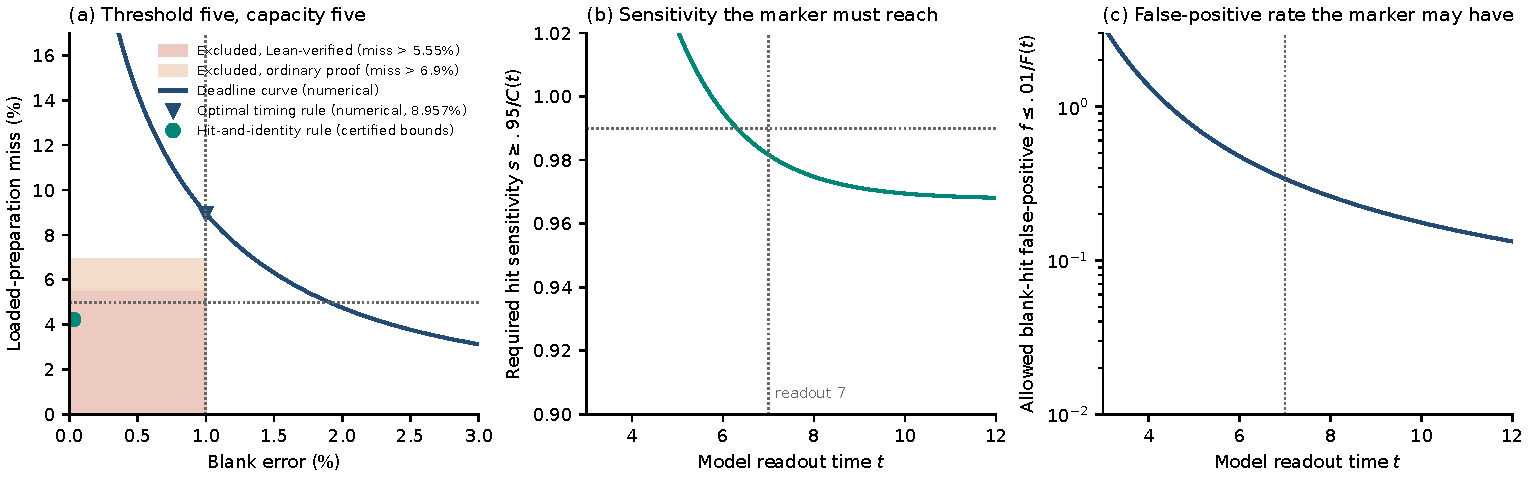
\includegraphics[width=\linewidth]{decision.pdf}
\caption{(a) The numerical deadline tradeoff at the nominal instance, the region forbidden to every crossing-time classifier (Lean-verified $5.55\%$ and ordinary-proof $6.9\%$), the numerical optimum, and the certified upper bounds of the hit-and-identity rule. (b) The hit-conditioned sensitivity a marker must reach for a $5\%$ miss, $s\ge.95/C(t)$, near its feasible boundary. (c) The blank-hit false-positive rate it may have for a $1\%$ blank error, $f\le.01/F(t)$. Curves are numerical illustrations; the shaded region and the marked point are theorems.}\label{fig:decision}
\end{figure}

\begin{proposition}[Label-neutral pipelines cannot repair the obstruction; ordinary proof]\label{prop:pipeline}
Suppose an observed datum $Y$ is generated from the complete crossing time by a Markov kernel $K(t,\dd y)$ that is the same under both labels. Then every classifier $\psi(Y)$ has exactly the errors of the crossing-time classifier $\phi(t)=\int\psi(y)K(t,\dd y)$. Hence every all-classifier lower bound of this section and of Section~\ref{sec:large} also holds for rules using $Y$.
\end{proposition}
\begin{proof}
$\phi$ is measurable with values in $[0,1]$ and $\E_i\psi(Y)=\E_i\phi(T)$ for $i=0,1$ by the tower property.
\end{proof}
This covers censoring at a finite horizon, timing noise, frame quantization, and an exogenous random global time change whose law does not depend on the label, including one with a ``never observed'' outcome. It does not require the transformed law to keep a monotone likelihood ratio, so the obstruction survives some random-clock mixtures for which deadline optimality itself needs separate analysis. It does not cover richer trajectory information or label-dependent clocks. An identity measurement escapes because it is not a label-neutral transformation of timing.

\subsection{Robustness}\label{sec:robust}
\begin{proposition}[Classwise discrepancy budgets; ordinary proof, scalar consequence Lean-verified]\label{prop:tv}
With $\TV(P,Q)=\sup_A|P(A)-Q(A)|$, suppose the actual blank and loaded crossing-time laws differ from the nominal ones by at most $\delta_0$ and $\delta_1$ in total variation. Then any rule with actual blank error at most $.01$ has actual miss greater than $.0555-5\delta_0-\delta_1$; exclusion at $5\%$ miss persists whenever $5\delta_0+\delta_1\le.0055$. For the fixed joint rule, classwise discrepancies $\eta_0,\eta_1$ give $\widetilde{\FP}_J<.0003+\eta_0$ and $\widetilde{\Miss}_J<.0422443+\eta_1$, so the limits survive if $\eta_0\le.0097$ and $\eta_1\le.0077557$.
\end{proposition}
\begin{proof}
For $0\le u\le1$, $\E_Pu=\int_0^1P(u>x)\dd x$, so $|\E_Pu-\E_Qu|\le\TV(P,Q)$. The nominal blank error is at most $.01+\delta_0$; apply \eqref{eq:dual} and transfer the miss back with error $\delta_1$ (\lean{discrepancy_budget}). Apply the same inequality directly to the joint rule.
\end{proof}
These are sufficient budgets, not measured discrepancies.

\begin{proposition}[A fixed-rate operating window; ordinary proof, exact computation, scalar consequence Lean-verified]\label{prop:robust}
Keep $R=h=5$ and let each fixed rate satisfy $q'_z\in[.98q_z,1.02q_z]$, the same vector in both classes. Let $\lambda\ge3.99$, let the actual readout time lie in $[6.99,7.01]$, and assume $f\le.01$, $s\ge.99$ uniformly. Then $\FP_J<.00032$ and $\Miss_J<.04525192$.
\end{proposition}
\begin{proof}
Couple holding times through common unit exponentials $E_z$: crossing from $n<h$ takes $\sum_{z\ge n}E_z/q'_z$, which decreases when any rate increases and when the initial state increases; couple Poisson loads by adding independent increments. By the source equivalence of Lemma~\ref{lem:holding}, $F_{q'}(t)\le F_q(1.02\times7.01)$ and $M_{q',\lambda}(t)\le M_{q,3.99}(.98\times6.99)$. Exact rational uniformization (Appendix~\ref{app:source}) gives $F_q(7.1502)<.032$, $M_{q,3.99}(6.8502)<.035$ and $e^{-3.99}<.019$, hence $C>1-.035-.019\times.032=.964392$ and, by \eqref{eq:frontier}, $\Miss_J\le1-.99\times.964392=565649/12500000=.04525192$ (\lean{robust_channel_arithmetic}).
\end{proof}
The inherited window of the companion manuscript is the same kind of statement for a usable timing rule: at $R=10$, $h=5$, the deadline $3.2$ meets both limits for every fixed rate vector within $2\%$, every loading at least $3.99$ and every actual time in $[3.19,3.21]$ (\lean{robust_guarantee}). Arbitrarily time-varying rates are outside both propositions.

\subsection{A larger threshold with a negligible initial atom}
At threshold five, $\Prob(N\ge5)=.371163$ of loaded reactions are positive at time zero. To remove this feature, take $R=h=20$ with $b=.01$, $g=1$, $\lambda=4$; then $\Prob(N\ge20)=1.0200522\times10^{-8}$. Table~\ref{tab:twenty} gives exact enclosures at times eight and ten. Every deadline is excluded, and by Corollary~\ref{cor:sharp} so is every crossing-time classifier, with miss above $.087$; at time ten the same channel premises give exactly the bounds \eqref{eq:joint}.

\begin{table}[htbp]\centering\small
\begin{tabular}{lrr}\toprule Quantity at $R=h=20$ & Numerical value & Exact enclosure\\\midrule
$F(8)$ & $.0134183123$ & $>.013$\\
$M(8)$ & $.0876466114$ & $>.087$\\
$F(10)$ & $.0297115009$ & $<.030$\\
$M(10)$ & $.0318119401$ & $<.032$\\
Joint blank error at 10 & $.0002971150$ & $<.0003$\\
Joint miss at 10 & $.0420271221$ & $<.0422443$\\\bottomrule
\end{tabular}
\caption{Threshold twenty. Numerical joint values use the fixture \eqref{eq:fixture}, which credits positive calls on empty loaded wells; the enclosures use \eqref{eq:frontier} and rational uniformization with $L=300$ terms. Neither threshold is a calibrated optical detection level.}\label{tab:twenty}
\end{table}

\section{Large thresholds: startup and terminal randomness}\label{sec:large}
Throughout this section $g=1$, $a=b/g>0$, $\lambda$ is fixed and $h\to\infty$; everything is ordinary proof or directed computation. Write $T_{R,h,n}$ for the crossing time from state $n<h$ at threshold $h$ and capacity $R$.

\subsection{The startup law}
\begin{lemma}[Beta law and gamma coupling; ordinary proof]\label{lem:beta}
Let $A_{h,n}=\sum_{z=n}^{h-1}E_z/(z+a)$. Then $e^{-A_{h,n}}\sim\Bet(n+a,h-n)$, and on an extension of the probability space there are $Z\sim\Gam(h+a,1)$ and $W_n\sim\Gam(n+a,1)$ with $A_{h,n}=\log Z-\log W_n$ exactly. Consequently $A_{h,n}-\log h\Rightarrow-\log W_n$.
\end{lemma}
\begin{proof}
$\E e^{-sA_{h,n}}=\prod_{z=n}^{h-1}\frac{z+a}{z+a+s}=\frac{\Gamma(n+a+s)\Gamma(h+a)}{\Gamma(n+a)\Gamma(h+a+s)}$ is the $s$th moment of $\Bet(n+a,h-n)$, and moments determine a law on $[0,1]$. Draw $Z\sim\Gam(h+a,1)$ independent of $e^{-A_{h,n}}$ and set $W_n=Ze^{-A_{h,n}}$; by the beta--gamma algebra \citep{lukacs1955}, $W_n\sim\Gam(n+a,1)$. Since $Z/(h+a)\to1$ in probability, the limit follows. $Z$ and $W_n$ are not independent, and nothing below uses independence between them.
\end{proof}
This is the logarithmic limit of the Yule process with immigration \citep{kendall1948}: after $\log h$ units of time a reaction started with $n$ units behaves like a $\Gam(n+a)$ effective initial mass. The blank member $\Gam(a)$ with $a=.01$ is extremely spread, and this spread is the whole difficulty of separating blanks from loaded reactions by timing. A large final count does not make a finite-founder startup deterministic. The limiting shift is minus the logarithm of a gamma variable; it is Gumbel only for shape one.

\subsection{Two resource regimes}
Under the coupling of Lemma~\ref{lem:holding}, $T_{R,h,n}=\frac{R}{R+a}[A_{h,n}+D_{R,h,n}]$ with $D_{R,h,n}=\sum_{z=n}^{h-1}E_z/(R-z)$.

\begin{theorem}[Growing reserve; ordinary proof]\label{thm:reserve}
Let $R=R(h)\ge h+1$ with $R-h\to\infty$, and let $d_h=\sum_{z=0}^{h-1}\frac{z}{(z+a)(R-z)}$. Then for every fixed $n$, $T_{R,h,n}-\log h-d_h\Rightarrow-\log W_n$ with $W_n\sim\Gam(n+a,1)$. If $R/h\to\rho>1$ then $d_h\to\log\frac{\rho}{\rho-1}$. For deadlines $t=\log h+d_h+s$,
\[
F(t)\to\Prob(W_0\ge e^{-s}),\qquad M(t)\to\sum_{n\ge0}\Prob(N=n)\Prob(W_n\le e^{-s}),
\]
the tradeoff of the undepleted source after a common delay.
\end{theorem}
\begin{proof}
Write $T=A_{h,n}+D'_n$ with $D'_n=\sum_{z\ge n}\frac{zE_z}{(z+a)(R-z)}$ (partial fractions). $\Var D'_n\le\sum_{z<h}(R-z)^{-2}\le(R-h)^{-1}\to0$ and $|\E D'_n-d_h|\le\sum_{z<n}(R-z)^{-1}\to0$, so $D'_n-d_h\to0$ in probability by Chebyshev; combine with Lemma~\ref{lem:beta}. For $\rho>1$, $d_h=\sum_{z<h}\frac1{R-z}-\sum_{z<h}\frac{a}{(z+a)(R-z)}$, whose first sum tends to $\log\frac\rho{\rho-1}$ and whose second is $O(\log h/(R-h))$. The error limits follow by continuity of the limit laws and dominated convergence over $n$.
\end{proof}

\begin{theorem}[Fixed headroom; ordinary proof]\label{thm:headroom}
Let $R=h+m$ with a fixed integer $m\ge0$. Then for every fixed $n$,
\[
T_{h+m,h,n}-2\log h\ \Rightarrow\ -\log W_n-\log Y_{m+1},
\]
with $W_n\sim\Gam(n+a,1)$ and $Y_{m+1}\sim\Gam(m+1,1)$ independent. For $m=0$, $-\log Y_1$ is standard Gumbel. For deadlines $t=2\log h+s$, $F(t)\to\Prob(W_0Y_{m+1}\ge e^{-s})$ and $M(t)\to\sum_n\Prob(N=n)\Prob(W_nY_{m+1}\le e^{-s})$.
\end{theorem}
\begin{proof}
Put $c=R/(R+a)$ and $k=\lfloor h/2\rfloor$. By \eqref{eq:holding}, $T/c=U_n+V+C_n$ with
\[
U_n=\sum_{z=n}^{k-1}\frac{E_z}{z+a},\qquad V=\sum_{z=k}^{h-1}\frac{E_z}{R-z}=\sum_{j=m+1}^{R-k}\frac{E'_j}{j},\qquad C_n=\sum_{z=n}^{k-1}\frac{E_z}{R-z}+\sum_{z=k}^{h-1}\frac{E_z}{z+a},
\]
where $E'_j=E_{R-j}$. The blocks $U_n$ and $V$ use disjoint exponentials and are independent. By Lemma~\ref{lem:beta} with $h$ replaced by $k$, $U_n-\log k\Rightarrow-\log W_n$; the transform $\E e^{-sV}=\prod_{j=m+1}^{R-k}\frac j{j+s}$ is that of $\Bet(m+1,R-k-m)$, so the same coupling gives $V-\log(R-k-m)\Rightarrow-\log Y_{m+1}$ with $Y_{m+1}\sim\Gam(m+1,1)$, and the two limits are independent. The remainder has $\E C_n\to2\log2$ (it equals $\log\frac R{R-k}+\log\frac hk+o(1)$) and $\Var C_n\le k/(R-k)^2+(h-k)/k^2=O(1/h)$, so $C_n-2\log2\to0$ in probability. Since $\log k+\log(R-k-m)+2\log2=2\log h+o(1)$ and $(1-c)O(\log h)\to0$, the claim follows. For $m=0$, $Y_1\sim\Ex(1)$ and $-\log Y_1$ is Gumbel \citep{erdosrenyi1961}.
\end{proof}
The mechanism is concrete. At $R=h$ the last transition has rate $q_{h-1}=g(a+h-1)/h\to g$, so its mean waiting time stays of order $1/g$ however large the threshold; at $R=2h$ the same rate is asymptotic to $gh/2$ and the waiting time vanishes. The last $m+1$ births before exhaustion contribute an independent $\Gam(m+1)$ variable in logarithmic time in addition to the startup shift. Random slowdown near an absorbing boundary is known in absorption-time asymptotics \citep{hathcock2022}; the point here is its exact form and its consequence for decisions. For $m=0$ the product law has the closed form
\begin{equation}\label{eq:bessel}
\Prob(W_nY_1\ge y)=\frac1{\Gamma(n+a)}\int_0^\infty w^{n+a-1}e^{-w-y/w}\dd w=\frac{2y^{(n+a)/2}}{\Gamma(n+a)}K_{n+a}(2\sqrt y).
\end{equation}

\begin{table}[htbp]\centering\footnotesize\setlength{\tabcolsep}{4pt}
\begin{tabular}{p{.30\linewidth}lrr}\toprule
Regime & Centered limiting time & Blank boundary $y$ & Miss at $1\%$ blank error\\\midrule
Growing reserve ($R-h\to\infty$, e.g.\ $R=2h$) & $-\log W_N$ & $.26505255$ & $3.96249\%$\\
Zero headroom ($R=h$) & $-\log W_N-\log Y_1$ & $.19364809$ & $10.91390\%$\\\bottomrule
\end{tabular}
\caption{Limiting tradeoffs at $a=.01$, $\lambda=4$ (numerical quadrature of the limit laws; the Bessel form \eqref{eq:bessel} and direct quadrature agree). Both regimes have $R/h=O(1)$; what decides is the remaining headroom at detection. Between them, headroom $m=1,2$ gives limiting miss $6.108\%$ and $5.027\%$, and $m\ge3$ gives a limiting window.}\label{tab:limits}
\end{table}

\subsection{A uniform theorem at every threshold of at least one million}
The limits above are qualitative. The following statement is quantitative, holds at every large threshold with explicit deadlines, and includes the identity repair. Let $k=\lfloor h/2\rfloor$, $\ell=h-k$, $c_h=h/(h+a)$, and
\begin{align}
\mu_-(h)&=\sum_{z=0}^{k-1}\frac1{h-z}+\sum_{z=k}^{h-1}\frac1{z+a},\qquad A_h=\log(k+a)+\log(\ell+1)+\mu_-(h),\label{eq:Ah}\\
\tau_-(h)&=c_h\bigl[A_h-\log(.15)\bigr],\qquad\tau_J(h)=c_h\bigl[A_h+\log200\bigr],\label{eq:tauminus}\\
\mu_+(h)&=\sum_{z=0}^{h-1}\frac{z}{(z+a)(2h-z)},\qquad\tau_+(h)=\log(h+a)+\mu_+(h)-\log(.3),\label{eq:tauplus}
\end{align}
all in units of $1/g$.

\begin{theorem}[Uniform large-threshold decision separation; ordinary proof with directed scalar certificates]\label{thm:big}
Let $a=.01$, $\lambda=4$, $\alpha=.01$, and let $h\ge10^{6}$ be an integer.
\begin{enumerate}[label=(\alph*)]
\item At $R=h$, $F(\tau_-)>.01086$ and $M(\tau_-)>.0563$; hence, by Corollary~\ref{cor:sharp}, every measurable randomized crossing-time classifier with blank error at most $.01$ has miss greater than $.0563$.
\item At $R=h$, a source-preserving identity measurement available at $\tau_J$ with blank-hit positive probability at most $.01$ and occupied-hit positive probability at least $.99$ gives a hit-and-positive rule with blank error below $.00085$ and miss below $.0413$. Its miss advantage over every admissible crossing-time classifier exceeds $1.5$ percentage points.
\item At $R=2h$, the deadline $\tau_+$ has blank error below $.009373$ and miss below $.048732$, so timing alone meets the limits.
\end{enumerate}
\end{theorem}
The proof is in Appendix~\ref{app:big}. Its ingredients are the couplings of Lemma~\ref{lem:beta} applied to the two blocks of Theorem~\ref{thm:headroom}, exponential concentration for the auxiliary gamma variables and for the weighted remainder, and a handful of scalar enclosures evaluated with directed rounding (Appendix~\ref{app:arith}). The earlier version of this argument in the companion manuscript used Chebyshev bounds whose $O(1/h)$ allowances forced $h\ge10^{8}$; replacing them by gamma Chernoff and weighted Bernstein bounds makes the allowances $e^{-ch}$ and lowers the sufficient threshold to $10^{6}$. That constant remains a convenient sufficient value; Theorem~\ref{thm:separation} covers $h=5$, Table~\ref{tab:twenty} covers $h=20$, and Figure~\ref{fig:large}(b) covers the range between numerically. Table~\ref{tab:times} displays the explicit times.

\begin{table}[htbp]\centering\footnotesize\setlength{\tabcolsep}{5pt}
\begin{tabular}{rrrr}\toprule
Threshold $h$ & $\tau_-$ (exhausted; separating) & $\tau_J$ (exhausted; joint readout) & $\tau_+$ (reserve; usable deadline)\\\midrule
$10^{6}$ & $29.52814$ & $32.92934$ & $15.71263$\\
$10^{8}$ & $38.73848$ & $42.13968$ & $20.31780$\\\bottomrule
\end{tabular}
\caption{Numerical evaluations of the exact formulas \eqref{eq:tauminus}--\eqref{eq:tauplus} in units of $1/g$. The times grow like $2\log h$ and $\log h$; no experimentally achieved turnaround follows without calibrating $g$ and the acquisition time. At $h=10^{6}$ the limiting conservative joint rule at product threshold $y=.005$ has miss $3.18421\%$ and blank error $.04089\%$ (numerical), which explains the margin the coarser proved bounds of part (b) leave.}\label{tab:times}
\end{table}

\begin{figure}[htbp]\centering

\includegraphics[width=\linewidth]{large_threshold.pdf}
\caption{(a) The limiting tradeoffs of Table~\ref{tab:limits} (curves and triangles, numerical) with the proved finite-threshold bounds of Theorem~\ref{thm:big} for every $h\ge10^{6}$ (square and circle). (b) Miss at the $1\%$ blank boundary of the optimal timing rule as the threshold grows, for fixed headroom $R=h,\dots,h+3$ and for $R=2h$, from Laplace-transform inversion \citep{talbot1979,abatewhitt2006} in the companion manuscript; dashed lines are the limits. Numerical.}\label{fig:large}
\end{figure}

\subsection{What the large-threshold behaviour resolves}
The scale objection is resolved within the declared family: an all-timing obstruction can persist at arbitrarily large thresholds, its cause being the order-one holding time of the last births before exhaustion together with the startup spread of the blank. It is not resolved by asserting that all physical assays operate in the exhausted regime. At $h=10^{6}$, fixed headroom of a few units means a threshold extremely close to the modeled capacity, and whether a detector, a signal map and a kinetic law place an assay there is an empirical question (Section~\ref{sec:discussion}). The reserve regime is as important to report as the obstruction: the same theory identifies conditions in which timing works, so it should not be read as universal necessity of an identity measurement. The displayed limits keep $a$ and $\lambda$ fixed while the threshold grows; they are not statements about every joint scaling of loading, background, resource and noise.

\section{Effective capacity: what intermediate observations identify}\label{sec:capacity}

\subsection{Exact endpoint nonidentification}
\begin{proposition}[Endpoint nonidentification; Lean-verified]\label{prop:nonident}
For blanks at threshold three, $(b,g,R)=(2,1,6)$ and $(8/3,2/3,4)$ have identical complete crossing-time probability measures.
\end{proposition}
\begin{proof}
The ordered pre-hit rates are $(2,5/2,8/3)$ and $(8/3,5/2,2)$. The crossing time is a sum of independent exponential holds with these rates, and convolution is commutative (\lean{endpoint_law_nonidentification}, an equality of measures, not of transforms or sampled values).
\end{proof}
Unlimited endpoint data cannot identify capacity in this family without restrictions; this is structural, not a lack of power. The example changes $a=b/g$ and does not assert nonidentification when $a$ is known, for loaded preparations, or for the intermediate trajectory. Figure~\ref{fig:capacity}(a) renders the equal laws.

\subsection{Paired calibrated waits}
Suppose $a$ is known, calibrated states $0\le i<j<R$ are observed, and each reaction has an unobserved constant positive clock multiplier $C_0$ so that its rates are $C_0q_z$. With independent unit exponentials, $D_z=E_z/(C_0g(a+z)(1-z/R))$, and the clock cancels pathwise in $D_j/D_i$ (\lean{clock_cancel}). Writing $q_i,q_j$ for the rates without $C_0$,
\begin{equation}\label{eq:paired}
p=\Prob(D_j>D_i)=\frac{q_i}{q_i+q_j},\qquad
\kappa=\frac{1-p}{p}\frac{a+i}{a+j}=\frac{R-j}{R-i},\qquad R=\frac{j-i\kappa}{1-\kappa},\quad0<\kappa<1
\end{equation}
(\lean{paired_exceedance_formula}, \lean{reconstruct_from_paired_probability}). For $a=.01$, $i=2$, $j=4$ the exact probabilities are $603/1004$, $335/736$ and $268/669$ at $R=5,7,10$. The innovations must have the declared independent exponential law; a random constant clock does not affect the ratio, but completion selection does (Section~\ref{sec:selection}).

\subsection{Calibrated blocks instead of resolved jumps}
Fluorescence does not resolve single count jumps. Let integers $k_0<k_1<k_2$ be calibrated states, $R>k_2-1$, and define the elapsed times across two consecutive blocks,
\begin{equation}\label{eq:blocks}
U_R=\sum_{z=k_0}^{k_1-1}\frac{E_z}{C_0g(a+z)(1-z/R)},\qquad V_R=\sum_{z=k_1}^{k_2-1}\frac{E_z}{C_0g(a+z)(1-z/R)},\qquad Q_R=\frac{V_R}{U_R}.
\end{equation}

\begin{theorem}[Ordered block ratios; ordinary proof, algebra Lean-verified]\label{thm:blocks}
$Q_R$ is invariant to the common positive clock. Under common positive innovations, $R_2>R_1>k_2-1$ implies $Q_{R_2}<Q_{R_1}$. Hence $p_r(R)=\Prob(Q_R>r)$ is nonincreasing in $R$ for every $r>0$.
\end{theorem}
\begin{proof}
Set $w_z(R)=R/((a+z)(R-z))$ and $m_z=w_z(R_2)/w_z(R_1)$. For $z<y$,
\[
m_z-m_y=\frac{R_2(R_2-R_1)(y-z)}{R_1(R_2-z)(R_2-y)}>0 .
\]
Expanding,
\[
V_{R_1}U_{R_2}-V_{R_2}U_{R_1}=\frac1{(C_0g)^2}\sum_{z=k_0}^{k_1-1}\sum_{y=k_1}^{k_2-1}E_zE_y\,w_z(R_1)w_y(R_1)(m_z-m_y)>0,
\]
a sum of positive terms (\lean{ordered_multiplier_term}, \lean{block_ratio_bound}). Dividing by the positive denominators orders the ratios; event inclusion orders the probabilities.
\end{proof}
For the exponential source the ordering probability is computable without simulation. With transient block generators $Q_U,Q_V$, initial rows $\alpha_U,\alpha_V$ and exit vector $d_U$, integrating the density of $U$ against the survival of $V$ at $rU$ gives the phase-type expression \citep{neuts1981}
\begin{equation}\label{eq:kronecker}
p_r(R)=(\alpha_U\otimes\alpha_V)\bigl[-(Q_U\oplus rQ_V)\bigr]^{-1}(d_U\otimes\one).
\end{equation}
The triangular generators have negative eigenvalues, and rational rates give exact rational linear systems: for blocks $[1,3)$ and $[3,5)$, $a=.01$, $r=1$, $p_1(7)=111503293/331058412$, and the values at $R=6,7,10,20,100$ are $.387971$, $.336809$, $.275672$, $.230952$, $.206321$ (Figure~\ref{fig:capacity}(b)).

\begin{theorem}[Strict probability ordering and unique inversion; ordinary proof]\label{thm:strict}
In the independent-exponential block experiment, for every $r>0$ the function $p_r$ is continuous and strictly decreasing on $(k_2-1,\infty)$, with $p_r(R)\to1$ as $R\downarrow k_2-1$ and a limit $p_r(\infty)\in(0,1)$ as $R\to\infty$. Hence every probability in $(p_r(\infty),1)$ determines a unique capacity in this family.
\end{theorem}
\begin{proof}
Fix $R_2>R_1$ and an innovation vector $e$ in the positive orthant; by Theorem~\ref{thm:blocks}, $Q_{R_2}(e)<Q_{R_1}(e)$. Multiplying only the late-block coordinates of $e$ by $s>0$ multiplies both ratios by $s$, so for $s$ in the nonempty interval $(r/Q_{R_1}(e),r/Q_{R_2}(e))$ the scaled vector satisfies $Q_{R_2}<r<Q_{R_1}$. Both ratios are continuous in $e$, so this holds on an open set, which has positive probability because the innovation vector has a positive density on the orthant. The event $\{Q_{R_1}>r\}$ therefore exceeds $\{Q_{R_2}>r\}$ by an event of positive probability: $p_r(R_2)<p_r(R_1)$. For continuity in $R$, $Q_R(e)$ is continuous in $R$ and $\{Q_R=r\}=\{V_R-rU_R=0\}$ is a hyperplane in $e$ with a nonzero normal, hence null; dominated convergence gives continuity of $p_r$. As $R\downarrow k_2-1$ the weight $w_{k_2-1}(R)$ diverges while $U_R$ stays finite, so $Q_R\to\infty$ almost surely and $p_r\to1$. As $R\to\infty$ every weight tends to $1/(a+z)$; the limiting ratio of two independent positive continuous variables exceeds $r$ with a probability strictly between zero and one. The intermediate value theorem gives unique inversion.
\end{proof}
The theorem does not make a finite-sample estimate precise, identify an unknown $a$, or recover the mean of a capacity mixture; if a larger source restricts capacities to a smaller interval, inversion is on that interval.

\begin{proposition}[Block ordering under general positive holding innovations; ordinary proof]\label{prop:general}
Suppose successive residence times admit a coupling $D_z(R,C_0)=A_z/(C_0v_zd_z(R))$ with $A_z>0$, $v_z>0$, $C_0>0$, where the joint law of $(A_z)$ is the same for the compared capacities; neither exponential marginals nor independence among the $A_z$ is required. If for $R_2>R_1$ the multipliers $m_z=d_z(R_1)/d_z(R_2)$ are strictly smaller at every late-block state than at every early-block state, then the block ratio cancels $C_0$ and strictly decreases from $R_1$ to $R_2$ pathwise. If moreover $(A_z)$ has a positive density on the positive orthant, the strict probability ordering of Theorem~\ref{thm:strict} holds as well.
\end{proposition}
\begin{proof}
Cancel $C_0$, write each weight at $R_2$ as its weight at $R_1$ times $m_z$, and expand the cross product as in Theorem~\ref{thm:blocks}; every summand is positive. The support argument of Theorem~\ref{thm:strict} uses only continuity and positive density.
\end{proof}
Concrete cases: serial multistep delays whose substeps share the factor $C_0d_z(R)$ (Erlang or other non-exponential residence times); correlated innovations with a capacity-independent joint law; arbitrary fixed state-specific baseline kinetics $v_z$; and several proportionally scaled resource pools, $d_z(R)=\prod_s(1-z/(c_sR))^{\gamma_s}$ with fixed $c_s,\gamma_s>0$, for which the inferred $R$ is a common scale rather than an identification of each pool. What these extensions preserve is the ordering; they do not preserve the closed form \eqref{eq:paired}, the phase-type formula \eqref{eq:kronecker} or the numerical timing certificates. Cases outside the proposition are direct diagnostics rather than vague realism caveats: an additive delay $L_z$ that does not scale with the clock, $D_z=A_z/(C_0q_z)+L_z$, generally does not cancel $C_0$ in a ratio; capacity-dependent innovation laws, state-specific drift and backward transitions are likewise excluded. A known time-dependent activity $q_z(t)=C_0c(t)q_z$ with $c>0$ is handled by the operational time $\Lambda(t)=\int_0^tc$: increments of $\Lambda$ replace clock-time increments and recover holds with rates $C_0q_z$; trajectories that do not complete within the finite total operational time must be retained as right-censored, and an unobserved completion must not be mapped to the finite value $\Lambda(\infty)$.

\subsection{Conditioning and depletion strength}
Put $A=a+i$, $B=a+j$, $d=j-i$, $D(R)=(A+B)R-(Ai+Bj)$. From \eqref{eq:paired},
\begin{equation}\label{eq:conditioning}
p(R)=\frac{A(R-i)}{D(R)},\qquad p_\infty=\frac A{A+B},\qquad p(R)-p_\infty=\frac{ABd}{(A+B)D(R)},\qquad p'(R)=-\frac{ABd}{D(R)^2}.
\end{equation}
Departure from unlimited capacity is $O(1/R)$ and sensitivity to an absolute change is $O(1/R^2)$: at large capacity the parameter is identified but poorly conditioned, which is a different phenomenon from Proposition~\ref{prop:nonident}. The depletion strength $\rho=1/R$ gives $p(\rho)=A(1-i\rho)/(A+B-(Ai+Bj)\rho)$ with $p'(0)=ABd/(A+B)^2>0$, a regular coordinate near unlimited capacity; an upper bound on $\rho$ stays informative when the capacity set is unbounded above (Figure~\ref{fig:capacity}(b)). For a target bracket $[R_-,R_+]$ let $\eps_p=\min\{p(R_-)-p(R),p(R)-p(R_+)\}$. By Hoeffding's inequality \citep{hoeffding1963}, $n\ge\log(2/\delta)/(2\eps_p^2)$ independent complete paired observations place the inverted point estimate in the bracket with probability at least $1-\delta$; to place an entire confidence interval centred at the estimate inside the bracket on its coverage event, use half the tolerance and four times the bound. With $a=.01$, $i=2$, $j=4$, $10\%$ relative precision and $\delta=.05$, the point-estimate bounds are $n=4{,}883$, $225{,}627$ and $9{,}911{,}503$ at $R=7$, $20$, $100$: sufficient scalings $O(R^2/\eps^2)$ for relative and $O(R^4/\eps^2)$ for absolute precision, for this fixed-state design and without any minimax claim.

\subsection{Plateau-normalized thresholds lose the leading capacity information}
A tempting preprocessing step chooses the count boundaries as fractions of each reaction's own plateau. In the source this means boundaries proportional to $R$, and it removes what the block method is meant to retain.

\begin{proposition}[Plateau normalization; ordinary proof]\label{prop:plateau}
Let $0<u_0<u_1<u_2<1$ and $k_r(R)=\lfloor u_rR\rfloor$ in the exponential source with fixed $a$. As $R\to\infty$,
\begin{gather*}
C_0g\,U_R\xrightarrow{P}L(u_0,u_1),\qquad C_0g\,V_R\xrightarrow{P}L(u_1,u_2),\\
L(u,v)=\int_u^v\frac{\dd x}{x(1-x)}=\log\frac v{1-v}-\log\frac u{1-u},
\end{gather*}
so $Q_R\to L(u_1,u_2)/L(u_0,u_1)$ in probability, a limit independent of capacity.
\end{proposition}
\begin{proof}
$\E(C_0gU_R)=\sum_{z=k_0}^{k_1-1}\frac1{(a+z)(1-z/R)}$ is a Riemann sum for the displayed integral; each coefficient is $O(1/R)$ and there are $O(R)$ independent unit-exponential terms, so the variance is $O(1/R)$. Chebyshev and the positive limit of the early block give the ratio limit; the late block is identical.
\end{proof}
For fractions $.2,.4,.6$ the limit is $.82678021$, and the ratios of expected block durations at $R=10^2,10^3,10^4,10^5$ are $.81814128$, $.82591487$, $.82669366$, $.82677156$ (Figure~\ref{fig:capacity}(c)). The proposition does not prove complete nonidentification, since finite-size corrections and fluctuation amplitudes may retain information, but it shows that plateau normalization cannot be substituted into Theorem~\ref{thm:blocks}: it moves the boundaries with $R$ and changes the experiment. The method should use externally calibrated fixed bands and propagate their uncertainty (Section~\ref{sec:signal}).

\begin{figure}[htbp]\centering
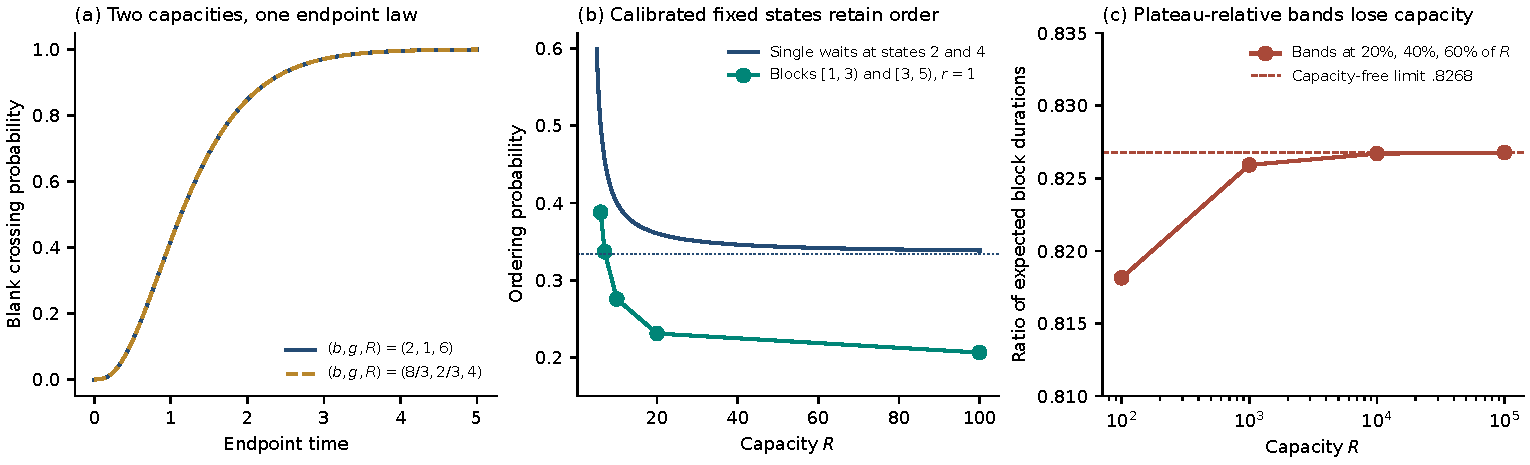
\includegraphics[width=\linewidth]{capacity.pdf}
\caption{(a) The exactly equal blank endpoint laws of Proposition~\ref{prop:nonident}, rendered numerically. (b) Calibrated single-wait and block ordering probabilities retain capacity information under their known-shape assumptions; the dotted line is $p_\infty$. (c) Plateau-relative bands at $20\%$, $40\%$, $60\%$ of capacity: the ratio of expected block durations converges to the capacity-free limit of Proposition~\ref{prop:plateau}.}\label{fig:capacity}
\end{figure}

\section{From signal to inference with incomplete observations}\label{sec:inference}

\subsection{Signal-to-state intervals}\label{sec:signal}
Begin with a declared measurement relation on a validated range, for instance $Y(t_m)=B+Kz(t_m)+\epsilon_m$ with baseline $B$, gain $K>0$ per calibrated state unit and readout error $\epsilon_m$; a known monotone nonlinear response can replace $Kz$ with interval inversion. If calibration provides $B\in[B_L,B_U]$, $K\in[K_L,K_U]$ with $K_L>0$, and a simultaneous error allowance $|\epsilon_m|\le\nu$ on the claimed event, then a recorded value $y$ implies
\begin{equation}\label{eq:state}
z_L=\max\Bigl(0,\frac{y-B_U-\nu}{K_U}\Bigr),\qquad z_U=\frac{y-B_L+\nu}{K_L},
\end{equation}
intersected with the state space and rounded outward for integer states; an empty intersection is a measurement/model incompatibility and must be reported, not clamped. For illustration only, a baseline in $[95,105]$ RFU, a gain in $[.9,1.1]\times10^{-3}$ RFU per unit, an allowance of $5$ RFU and a reading of $1110$ RFU give $z\in[909{,}091,\ 1{,}133{,}333]$: a nominal million-unit crossing is not a precisely calibrated million-state crossing, and if the scientific distinction concerns a few units of headroom this calibration is insufficient. For each fixed calibrated threshold $k$, a frame is certainly below when $z_U<k$ and certainly at or above when $z_L\ge k$; under the monotone latched count model the last certainly-below and first certainly-above frames bracket the crossing time, an infinite upper endpoint is retained when no above-threshold frame is certified, and initially-above cases form their own category. If $\tau_{k_r}\in[L_r,U_r]$ then consecutive block durations satisfy
\begin{equation}\label{eq:blockbounds}
\Delta_r\in\bigl[\max(0,L_{r+1}-U_r),\ U_{r+1}-L_r\bigr].
\end{equation}
Shared crossing times make neighbouring block bounds dependent; the inference below does not require independence between them. Crossings bracketed by $[2,2.1]$, $[3.5,3.6]$ and $[4.9,5.0]$ give $U\in[1.4,1.6]$ and $V\in[1.3,1.5]$, and the comparison $V>U$ is unresolved; replacing the intervals by midpoints would discard exactly the uncertainty that matters. A pointwise calibration band is not a simultaneous band over thousands of frames; a shared calibration failure probability $\delta_{\rm cal}$ is combined with the inference failure allowance by a union bound, and per-reaction bad-bracket probabilities are handled in Theorem~\ref{thm:censor}.

\subsection{The selection failure}\label{sec:selection}
For $a=.01$, $i=2$, $j=4$, $R=7$, the full-cohort ordering probability is $p=335/736=.455163$ for every constant clock. Conditioning on the sum-of-waits completion event $D_i+D_j\le1$ changes it to $.491088$, $.479803$ and $.459864$ at clock multipliers $.4$, $1$ and $3$: with rates including the clock, the selected numerator is $\int_0^{1/2}q_ie^{-q_iu}(e^{-q_ju}-e^{-q_j(1-u)})\dd u$ and the completion probability $\int_0^1q_ie^{-q_iu}(1-e^{-q_j(1-u)})\dd u$ (Figure~\ref{fig:censoring}(a)). Pathwise cancellation before selection does not imply invariance in a selected subpopulation, so deleting slow observations defeats the method; the remedy is to keep them.

\subsection{Censoring-safe partial information}
\begin{theorem}[Censoring-safe confidence sets; ordinary proof]\label{thm:censor}
Suppose genuine recorded bounds give $U\in[L_U,U_U]$ and $V\in[L_V,U_V]$, with infinite upper endpoints allowed. For $r>0$ call an observation certain positive if $L_V>rU_U$, certain negative if $U_V\le rL_U$, and unknown otherwise. If the first two categories have probabilities $\pi_+,\pi_-$ then
\begin{equation}\label{eq:category}
\pi_+\ \le\ p=\Prob(V>rU)\ \le\ 1-\pi_- .
\end{equation}
For $n$ independent observations with the same latent $p$ and possibly nonidentical censoring, with counts $n_+,n_-$, with probability at least $1-\delta$,
\begin{equation}\label{eq:confidence}
p\in\Bigl[\max\Bigl(0,\frac{n_+}n-e_n\Bigr),\ \min\Bigl(1,1-\frac{n_-}n+e_n\Bigr)\Bigr],\qquad e_n=\sqrt{\frac{\log(2/\delta)}{2n}} .
\end{equation}
Independence of the censoring from the latent waits is not needed. If the bracket of observation $i$ is invalid with probability at most $\epsilon_i$, the statement holds with $e_n$ replaced by $e_n+n^{-1}\sum_i\epsilon_i$.
\end{theorem}
\begin{proof}
The certain-positive event lies inside $\{V>rU\}$ and the certain-negative event inside its complement, which proves \eqref{eq:category}; the width of the interval equals the unknown mass, and it is sharp given only the category probabilities, since assigning every unknown outcome to either latent class attains an endpoint. For \eqref{eq:confidence}, apply one-sided Hoeffding bounds \citep{hoeffding1963} to the two independent indicator sums around their average expectations, each with tail $\delta/2$, and use a union bound; each average expectation obeys \eqref{eq:category}. With invalid brackets, a certain-positive call can exceed the true positive event only on the bad-bracket event, so the category probability can exceed $p$ by at most $\epsilon_i$, and similarly for certain negatives; average over $i$.
\end{proof}
Observation vectors must be independent across reactions; shared run effects need a justified independent unit or a conditional model. A shared nuisance is harmless when, conditionally on it, the observations are independent with the same latent $p$, as for a shared constant clock under the exact invariance model; arbitrary run effects are not. Continuous latent waits permit the displayed strict and nonstrict rules; recording atoms need conservative boundary handling.

\subsection{Capacity sets}
For single waits, transform the confidence set by \eqref{eq:paired}, intersecting with $0<\kappa<1$; since $\kappa$ decreases in $p$ and increases in $a$, an uncertain $a\in[a_L,a_U]$ has conservative extreme values at $(p_U,a_L)$ and $(p_L,a_U)$. An empty physical intersection is a model incompatibility at the stated confidence level; an interval reaching $\kappa=1$ has unbounded upper capacity; $\kappa=0$ corresponds to $R=j$, excluded for a positive dwell at $j$. For blocks, take $\{R:p_r(R)\in[p_L,p_U]\}$ with validated enclosures of \eqref{eq:kronecker}; Theorem~\ref{thm:strict} makes this an interval, and Theorem~\ref{thm:blocks} alone still supports brackets. The output may be a finite interval, a one-sided bound, the whole admissible domain, or an empty set, and none of these is to be replaced by a forced point estimate.

\begin{table}[htbp]\centering\small
\begin{tabular}{lrrrrll}\toprule
Simulation & $R$ & $n_+$ & $n_-$ & Unknown & $95\%$ set for $p$ & $95\%$ capacity set\\\midrule
Resolved waits & 7 & 1752 & 2229 & 19 & $[.416527,.464223]$ & $[6.745,8.715]$\\
Short follow-up & 7 & 478 & 639 & 2883 & $[.098027,.861723]$ & $[4.175,\infty)$\\
Large capacity & 100 & 1367 & 2600 & 33 & $[.320277,.371473]$ & $[15.167,\infty)$\\\bottomrule
\end{tabular}
\caption{Prespecified seeded simulations (seed 20260916), $n=4000$ each, $a=.01$, $i=2$, $j=4$, clocks drawn independently from $\{.4,1,3\}$; every observation is retained. Each designated dwell has its own horizon (8 with frame width $.002$ in rows one and three; $.12$ with frame width $.05$ in row two), unlike the sum-of-waits selection of Section~\ref{sec:selection}. The last row gives $\rho\in[0,.06594]$ although the capacity set is unbounded. Simulations illustrate the theorem; they neither prove coverage nor validate anything empirically.}\label{tab:simulation}
\end{table}

\begin{figure}[htbp]\centering
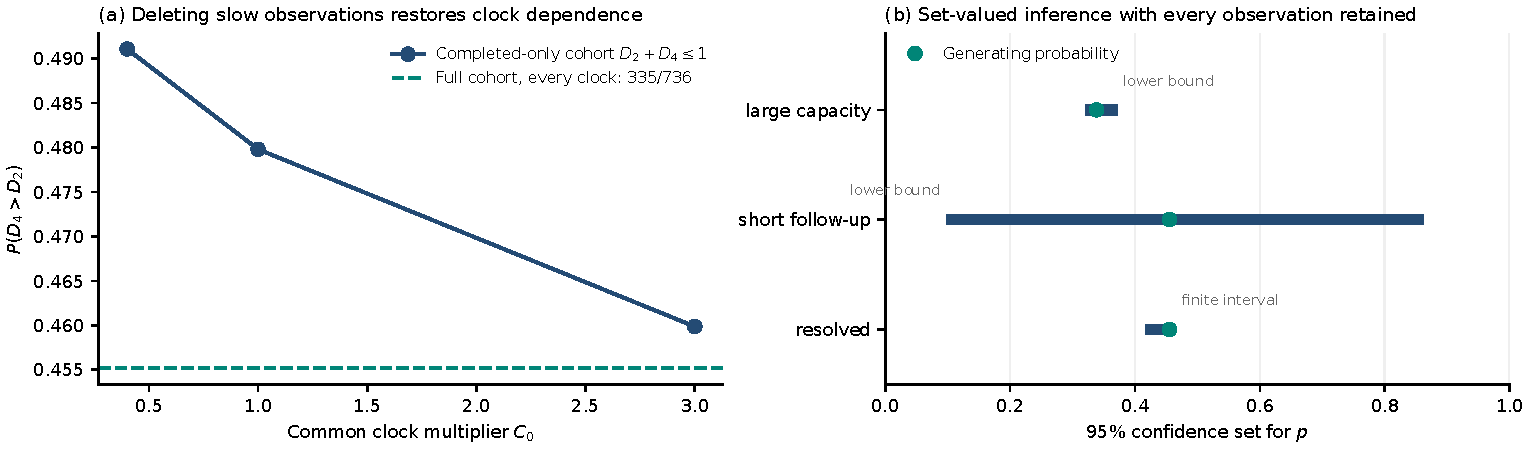
\includegraphics[width=\linewidth]{censoring.pdf}
\caption{(a) Completion selection restores clock dependence (Section~\ref{sec:selection}). (b) Probability confidence sets of Table~\ref{tab:simulation} with the generating probabilities and the returned status.}\label{fig:censoring}
\end{figure}

\subsection{A usable decision procedure}\label{sec:procedure}
Suppose $[F_L,F_U]$ and $[M_L,M_U]$ simultaneously contain both errors over the candidate readouts. A readout is \emph{usable} if $F_U\le\alpha$ and $M_U\le\beta$; \emph{excluded} if $F_L>\alpha$ or $M_L>\beta$; and \emph{unresolved} otherwise. Containment makes the first two verdicts sound, selection among simultaneously covered candidates preserves the guarantee, and for an actual time in $[t_-,t_+]$ the blank error is bounded at $t_+$ and the miss at $t_-$ (\lean{usable_sound}, \lean{excluded_sound}, \lean{selected_time_sound}, \lean{jitter_endpoints}). The inherited capacity-ten instance at time $3.2$ is usable; the coarse bands $F\in[0,.02]$, $M\in[0,.1]$ leave that same instance unresolved; and at capacity five the miss lower bound at time five excludes that deadline (\lean{three_decision_examples}). Wide evidence and physical impossibility are different verdicts, and collecting better evidence can resolve the former but not the latter.

A researcher-facing version of the analysis, implementable without reading any formal proof, is the following.
\begin{enumerate}[label=(\arabic*)]
\item Declare the blank and loaded populations, the loading model including empties, the independent unit, the error limits, and the available readout times and measurements.
\item Retain noncrossers and incomplete observations. Obtain model or empirical error enclosures for each candidate time, including the source uncertainty and the timing allowance, and return usable, excluded or unresolved.
\item If every deadline is excluded, the exclusion applies to every crossing-time classifier (Theorem~\ref{thm:mlr}). Evaluate a candidate identity channel through $fF(t)\le\alpha$ and $sC(t)\ge1-\beta$ with hit-conditioned $f$ and $s$, and its acquisition time; if a change of reserve is within scope, compare the resource regimes of Section~\ref{sec:large}.
\item For mechanism questions, convert calibrated frames into state and crossing intervals \eqref{eq:state}--\eqref{eq:blockbounds}, keep the unknown category, and return a probability confidence set and its capacity or depletion-strength image.
\item Report one finite interval and one one-sided or unresolved case explicitly, and state which additional information would narrow the latter.
\end{enumerate}
For a prespecified rule and independent Bernoulli trials, zero errors in $n$ trials give the one-sided upper bound $1-\gamma^{1/n}$ at tail probability $\gamma$ \citep{clopperpearson1934,hanley1983}. Allocating $\gamma=.025$ to each error, $368$ blank and $72$ loaded zero-error trials give simultaneous $1\%$ and $5\%$ upper limits, and a $.03\%$ bound needs $12{,}295$ eligible trials. These are planning calculations. Conditional marker calibration uses the hit-conditioned denominator, and selecting a time or a rule from the same data needs simultaneous coverage or an independent evaluation set.

\section{Scope and the empirical frontier}\label{sec:discussion}
Three consequences change an analysis. An all-rule timing certificate ends futile cutoff tuning, and the deadline-optimality theorem says that no cleverer function of the same datum will do better. Equal endpoint laws defeat unlimited endpoint replication, while labeled intermediate observations retain rate order, and the strict inversion theorem tells what a block probability determines. Incomplete observations support an honest one-sided capacity bound instead of a biased complete-case estimate.

The results are conditional on the declared source, and Table~\ref{tab:bridge} lists what connects each model object to a measurement. The primary empirical question is whether a realizable identity measurement meets the hit-conditioned bounds while preserving the total-count source across its operating range; the assumed $99\%/1\%$ capabilities should not be called standard performance without physical evidence. Calibrated state intervals with propagated band uncertainty, a constant within-reaction clock, and the identity of the consumed resource behind the effective capacity are the other substantive assumptions; an effective capacity fit is not a mechanism, and inversion of a capacity mixture does not recover its mean. The headroom prediction of Section~\ref{sec:large} is testable: under a controlled resource intervention with matched blanks, known loading, all trajectories retained and independent run labels, the sensitivity--blank tradeoff should change with the remaining headroom at detection and should disappear when the reserve is large, whereas a common clock change only shifts all crossing times.

\begin{table}[htbp]\centering\small
\begin{tabular}{>{\raggedright\arraybackslash}p{.17\linewidth}>{\raggedright\arraybackslash}p{.29\linewidth}>{\raggedright\arraybackslash}p{.46\linewidth}}\toprule
Model object & Candidate measurement & Required bridge\\\midrule
State $z$, threshold $h$ & Effective product amount & Calibrated signal/state map with uncertainty \eqref{eq:state}; small thresholds are illustrative.\\
Capacity $R$, headroom & Growth suppression near detection & Rate-law fit; separate mechanistic evidence for a consumed resource; the headroom intervention above.\\
Scale $g^{-1}$ & Physical elapsed time & Rate calibration and acquisition duration.\\
Poisson loading & Target allocation & Loading distribution and a denominator including empties.\\
Identity channel & Product-sensitive readout & Hit-conditioned errors against an independent product-identity reference; availability at the readout time; no kinetic effect.\\
Block intervals & Calibrated signal crossings & State bounds, latching convention, frame resolution, retained missingness.\\
Independent unit & Reaction, run, batch & Independent identifiers or a justified conditional model.\\\bottomrule
\end{tabular}
\caption{Source-to-observation requirements. No row is empirically established by the theoretical results.}\label{tab:bridge}
\end{table}

Open problems. (1) A measured interpretation of effective capacity, background and growth, and the headroom intervention. (2) Sharper constants: the certified $5.55\%$ and $6.9\%$ against the numerical $8.96\%$, and the sufficient threshold $10^{6}$. (3) Formalization of Theorem~\ref{thm:mlr}, of the holding-time and beta--gamma arguments, and of the full probabilistic block theorem, which would raise Sections~\ref{sec:large}--\ref{sec:capacity} to the evidence level of Theorem~\ref{thm:separation}. (4) Sources with unequal target and background kinetics, activation delays, extinction, time-dependent rates of unknown form, and adaptive stopping, each of which changes the source and needs its own separation analysis. (5) Specimen-level rules that aggregate several reactions.

\section{Verification and reproducibility}\label{sec:verification}
\paragraph{Lean-verified.}
The formal development lives in the namespaces \lean{DiagnosticWindows} and \lean{AssayInformation} of a frozen Lean~4 project (toolchain \lean{leanprover/lean4:v4.30.0}, pinned Mathlib manifest with SHA-256 prefix \texttt{a8df0b60}), compiled with warnings treated as errors; every strict receipt lists only the axioms \lean{propext}, \lean{Classical.choice} and \lean{Quot.sound}, and no \lean{sorry}, asserted source bridge or unchecked numerical solver closes any formal root. The combined declaration \lean{AssayInformation.main} (source SHA-256 prefix \texttt{6fce3549}, 34 imported modules, 67 s) asserts: the all-classifier obstruction $\Miss>111/2000$ for every measurable $\phi$ with values in $[0,1]$ and $\FP\le1/100$; the joint fixture bounds $\FP_J<3/10000$ and $\Miss_J<422443/10^{7}$; the three decision-band examples; the endpoint-law equality; and the paired-observation reconstruction identity. The extension modules \lean{DecisionGap} (SHA-256 prefix \texttt{d2c3b4ac}) and \lean{BlockRatio} (\texttt{c777cd3d}) supply the strict gap, the two scalar robustness consequences and the block algebra. Appendix~\ref{app:map} maps claims to declarations.

\paragraph{Ordinary proof.}
Lemma~\ref{lem:holding} and the source equivalence of Appendix~\ref{app:source}; Theorem~\ref{thm:mlr} and Corollary~\ref{cor:sharp}; Propositions~\ref{prop:floor}, \ref{prop:pipeline}, \ref{prop:tv} and \ref{prop:robust} (beyond their compiled scalar parts); all of Section~\ref{sec:large}, including Theorem~\ref{thm:big} with Appendices~\ref{app:big}--\ref{app:arith}; Theorems~\ref{thm:blocks} (beyond its compiled algebra), \ref{thm:strict} and \ref{thm:censor}; Propositions~\ref{prop:general} and \ref{prop:plateau}. None of these is labeled Lean-verified.

\paragraph{Exact and directed computation.}
Every printed enclosure of Sections~\ref{sec:timing} and \ref{sec:large} and of Appendices~\ref{app:certificate}--\ref{app:arith}, the rational block probabilities, the capacity sets and the design counts are replayed by \path{check_paper.py} (102 named checks, exact fractions or Python \texttt{decimal} with explicit rounding directions, cross-checked with \texttt{mpmath}); it also regenerates the coefficient table of Appendix~\ref{app:certificate}.

\paragraph{Numerical illustration.}
The deadline curves, the optimum $t_\alpha=4.4594$ with miss $8.9566\%$, the limit-law values of Tables~\ref{tab:limits} and \ref{tab:times}, the convergence panel of Figure~\ref{fig:large}(b), the numerical column of Table~\ref{tab:twenty}, the selection regression and the seeded simulations of Table~\ref{tab:simulation}. The figures are produced by \path{make_figures.py}. \RepositoryNote

\appendix

\section{The uniformized source and the holding-time equivalence}\label{app:source}
Let $Q$ be the $(h+1)$-state generator with $Q_{zz}=-q_z$, $Q_{z,z+1}=q_z$ for $z<h$ and a zero absorbing row at $h$. For $\nu\ge\max_zq_z$ put $P=I+Q/\nu$, a stochastic matrix; the uniformized transition matrix is $K_t=e^{-\nu t}\sum_{k\ge0}\frac{(\nu t)^k}{k!}P^k=e^{tQ}$ \citep{jensen1953}. The independent-holding-time construction has the same generator, since exponential memorylessness gives the first-step transition and holding rate at every state; its transition matrix solves $K'_t=K_tQ$, $K_0=I$, and uniqueness of this finite linear system identifies it with $e^{tQ}$. Writing $S_n(t)=\Prob(T>t\mid X_0=n)$, one has $S_h=0$, $S_n(0)=1$ for $n<h$, $S'_n=-q_nS_n+q_nS_{n+1}$, and for distinct rates
\begin{equation}\label{eq:spectral}
S_n(t)=\sum_{i=n}^{h-1}c_{ni}e^{-q_it},\qquad c_{ni}=\frac{\prod_{j=n}^{h-1}q_j}{q_i\prod_{j=n,\,j\ne i}^{h-1}(q_j-q_i)},
\end{equation}
with $F(t)=1-S_0(t)$ and $M(t)=e^{-\lambda}\sum_{n<h}\frac{\lambda^n}{n!}S_n(t)$; the omitted terms $N\ge h$ are the initial atom. The concrete Lean source uses $\nu=5/2$ and rational transition probabilities at threshold five, and verifies the spectral identities algebraically inside the uniformized law. For rigorous enclosures at arbitrary rational times, compute $P^k\one_{z<h}$ recursively with exact fractions, truncate the Poisson series at $L$ terms, bound the omitted tail through the enclosure $1/(A_L(x)+R_L(x))\le e^{-x}\le1/A_L(x)$ with $A_L(x)=\sum_{k\le L}x^k/k!$ and $R_L(x)=\frac{x^{L+1}}{(L+1)!}\frac1{1-x/(L+2)}$, and combine with the finite loading sum. The fixed-rate window uses $L=200$ at the effective times $1.02\times7.01$ and $.98\times6.99$ with loading $3.99$; the threshold-twenty example uses $L=300$ at times eight and ten.

\section{The sign certificate for the timing obstruction}\label{app:certificate}
For \eqref{eq:nominal} the rates in state order are $(5,404,603,602,401)/500$. Differentiating \eqref{eq:spectral},
\[
f_0(t)=\sum_iq_ic_{0i}e^{-q_it},\qquad f_1(t)=e^{-4}\sum_iq_iB_ie^{-q_it},\qquad B_i=\sum_{n=0}^4\frac{4^n}{n!}c_{ni}.
\]
With $x=e^{-t/500}$, $f_1(t)-5f_0(t)=x^5P(x)$ where
\begin{gather*}
P(x)=-A+Bx^{396}-Dx^{399}+Ex^{597}-Gx^{598}=x^{396}H(x)-A,\\
H(x)=B-Dx^3+x^{201}(E-Gx) .
\end{gather*}
Table~\ref{tab:coeff} gives outward terminating-decimal enclosures of the five signed coefficients, reconstructed from the rational $c_{ni}$ and an enclosure of $e^{-4}$; substituting lower endpoints gives $P_-$ and upper endpoints $P_+$, with $P_-\le P\le P_+$ for $x\ge0$.
\begin{table}[htbp]\centering\small
\begin{tabular}{rrr}\toprule Exponent & Lower coefficient & Upper coefficient\\\midrule
0 & -0.051936436911 & -0.051936436910\\
396 & 133.156300607087 & 133.156300607088\\
399 & -135.013385312608 & -135.013385312607\\
597 & 127.123028975878 & 127.123028975879\\
598 & -125.057323647968 & -125.057323647967\\
\bottomrule\end{tabular}

\caption{Outward coefficient enclosures (regenerated by \texttt{check\_paper.py}); the formal proof uses the same source identities with a slightly different exact enclosure and the same four-cell argument.}\label{tab:coeff}
\end{table}
\emph{Late region.} Put $v=9901/10000$. The upper coefficients satisfy $D,G\ge0$, $396B-399Dv^3\ge0$, $597E-598Gv\ge0$ and $P_+(v)<-.0021371$; since $P'_+(x)=x^{395}\{396B-399Dx^3+x^{201}(597E-598Gx)\}\ge0$ on $[0,v]$, $P_+<0$ there. For $t\ge5$, $e^{t/500}\ge1.01$ gives $x\le100/101<v$. \emph{Early region.} Divide $[.992,1]$ at $.994,.996,.998$. On a cell $[l,u]$ the lower coefficients satisfy $D,G\ge0$, $E-Gu\ge0$ and $H'(x)\le-3Dl^2+201u^{200}(E-Gl)-Gl^{201}<0$; also $H(u)>0$, so $P_-(x)\ge l^{396}H(u)-A$, which exact checks bound below by $.0061843$, $.0313825$, $.0503130$ and $.0424808$ on the four cells (with $H'$ bounded above by $-238.51$, $-183.57$, $-112.10$, $-21.56$). For $0\le t\le4$, $x\ge1-t/500\ge.992$. This proves \eqref{eq:signs}; the enclosures $F(4)>.0073$ and $M(5)>.069$ come from Appendix~\ref{app:source}. The displayed decimals are conservatively rounded reports of exact rational checks, and their numerical appearance is not the evidence.

\section{Proof of Theorem~\ref{thm:big}}\label{app:big}
Fix $a=.01$, $\eps=.01$, $n_*=25$, and let $h\ge10^{6}$. All times are in units of $1/g$.

\paragraph{Concentration inequalities.}
For $Z\sim\Gam(s,1)$ with real $s>0$ and $0<\eps\le1$, exponential Markov bounds with the optimal parameters $t=1-e^{-\eps}$ and $t=e^{\eps}-1$ give
\begin{equation}\label{eq:chernoff}
\Prob\bigl(|\log(Z/s)|>\eps\bigr)\le e^{-s(e^{\eps}-1-\eps)}+e^{-s(e^{-\eps}-1+\eps)}\le2e^{-s\eps^2/3},
\end{equation}
using $e^{\eps}-1-\eps\ge\eps^2/2$ and $e^{-\eps}-1+\eps\ge\eps^2/2-\eps^3/6\ge\eps^2/3$. For independent unit exponentials and $S=\sum_ra_r(E_r-1)$ with $0\le a_r\le b_*$ and $V=\sum_ra_r^2$,
\begin{equation}\label{eq:bernstein}
\Prob(|S|\ge\eps)\le2\exp\Bigl[-\frac{\eps^2}{2(V+b_*\eps)}\Bigr]:
\end{equation}
for $0<t<1/b_*$, $\log\E e^{tS}=\sum_r[-\log(1-ta_r)-ta_r]\le\frac{t^2V}{2(1-tb_*)}$, and $t=\eps/(V+b_*\eps)$ gives the upper tail; the lower tail is smaller since $-\log(1+x)+x\le x^2/2$ \citep{boucheron2013}.

\paragraph{Elementary bounds on the limit laws.}
(i) $99\le\Gamma(a)\le100$: with $X\sim\Ex(1)$, $\Gamma(a)=\E[X^a]/a$, concavity gives $\E X^a\le1$, and $X^a\ge1+a\log X$ with $\E\log X\ge-1$ gives $\E X^a\ge1-a$. (ii) From $w^a\le1-a+aw$,
\begin{equation}\label{eq:blankup}
\Prob(\Gam(a,1)\ge y)\le.01E_1(y)+\frac{e^{-y}}{9900},\qquad E_1(y)=\int_y^\infty\frac{e^{-w}}w\dd w .
\end{equation}
(iii) For $n\ge1$, $\Gam(n+a)$ stochastically dominates $\Gam(n)$ and $\Prob(\Gam(n,1)\le y)\le y^n/n!$; bounding the $n=0$ term by one,
\begin{equation}\label{eq:missup}
\sum_{n\ge0}\Prob(N=n)\Prob(\Gam(n+a,1)\le y)\le e^{-4}\sum_{n\ge0}\frac{(4y)^n}{(n!)^2}.
\end{equation}
(iv) For $Y\sim\Ex(1)$ independent of $W\sim\Gam(a,1)$, since $.97^{100}<.05$ gives $w^a\ge.97$ on $w\ge.05$,
\begin{equation}\label{eq:blanklow}
\Prob(WY\ge y)=\frac1{\Gamma(a)}\int_0^\infty w^{a-1}e^{-w-y/w}\dd w\ge.0097\int_{.05}^{10}\frac{e^{-w-y/w}}w\dd w .
\end{equation}
(v) For $W_n\sim\Gam(n+a,1)$, by $1-e^{-u}\ge u/(1+u)$ and Jensen,
\begin{equation}\label{eq:misslow}
\Prob(W_nY\le y)=\E\bigl[1-e^{-y/W_n}\bigr]\ge\E\Bigl[\frac y{W_n+y}\Bigr]\ge\frac y{n+a+y}.
\end{equation}
(vi) For $n\ge2$, $\Prob(W_nY\le v)=\E[1-e^{-v/W_n}]\le v\E[W_n^{-1}]=\frac v{n+a-1}\le\frac v{n-1}$; for $n=1$, $W_1$ dominates $\Ex(1)$, and a product of two independent unit exponentials is at most $v$ only if one factor is at most $\sqrt v$, so $\Prob(W_1Y\le v)\le2\sqrt v$. (vii) $\Prob(N>25)\le e^{-4}\frac{4^{26}}{26!}(1-\frac4{27})^{-1}<3\times10^{-13}$.

\paragraph{The exhausted source.}
With $c_h=h/(h+a)$, $k=\lfloor h/2\rfloor$, $\ell=h-k$, Lemma~\ref{lem:holding} gives $T_{h,h,n}/c_h=U_n+V_h+C_n$ with $U_n=\sum_{z=n}^{k-1}E_z/(z+a)$, $V_h=\sum_{z=k}^{h-1}E_z/(h-z)$ and $C_n=\sum_{z=n}^{k-1}E_z/(h-z)+\sum_{z=k}^{h-1}E_z/(z+a)$. For $n\le25$ the couplings of Lemma~\ref{lem:beta} give $U_n=\log Z_1-\log W_n$ and $V_h=\log Z_2-\log Y$, with $Z_1\sim\Gam(k+a,1)$, $Z_2\sim\Gam(\ell+1,1)$, $W_n\sim\Gam(n+a,1)$, $Y\sim\Ex(1)$, and $W_n$, $Y$ independent; the $Z$'s need not be independent of anything, and only a union bound is used. Every coefficient of $C_n$ is at most $1/k$ and there are at most $h$ terms; with $k\ge(h-1)/2$ and $h\ge10^{6}$, $V\le h/k^2\le4.01/h$, $b_*\le1/k\le2.01/h$, and $k+a,\ \ell+1\ge h/2.01$; also $|\E C_n-\mu_-(h)|\le25/(h-24)$. Applying \eqref{eq:chernoff} to $Z_1,Z_2$ and \eqref{eq:bernstein} to $C_n-\E C_n$ with $\eps=.01$, the failure probability is at most
\begin{equation}\label{eq:deltaminus}
\Delta_-(h)=4e^{-h/60300}+2e^{-h/80602}<10^{-5},
\end{equation}
decreasing in $h$ and equal to $8.43\times10^{-6}$ at $10^{6}$. Outside the failure event, since $3\eps+25/(h-24)<.0301$,
\begin{equation}\label{eq:goodminus}
\bigl|T_{h,h,n}/c_h-A_h+\log(W_nY)\bigr|<.0301\qquad(n\le25).
\end{equation}

\emph{(a) Timing obstruction.} At $\tau_-$, on the good event, $W_0Y\ge.155>.15e^{.0301}$ forces $T\le\tau_-$, and $W_nY\le.145<.15e^{-.0301}$ forces $T>\tau_-$. Hence, keeping only loads $n\le5$ in the second bound and using \eqref{eq:misslow},
\[
F(\tau_-)\ge\Prob(W_0Y\ge.155)-\Delta_-,\qquad M(\tau_-)\ge e^{-4}\sum_{n=0}^5\frac{4^n}{n!}\frac{.145}{n+.155}-\Delta_- .
\]
The directed computation of Appendix~\ref{app:arith} gives $\Prob(W_0Y\ge.155)>.01087$ and a finite sum exceeding $.056383$, so $F(\tau_-)>.01086>.01$ and $M(\tau_-)>.056373>.0563$. Thus $\tau_-$ is a separating time, every deadline is excluded, and Corollary~\ref{cor:sharp} gives miss greater than $.0563$ for every crossing-time classifier with blank error at most $.01$.

\emph{(b) Identity repair.} At $\tau_J$, put $y=1/200$. On the good event a missed occupied reaction with load $n\ge1$ has $W_nY<ye^{.0301}<v:=.00516$. By (vi), (vii) and the exact bounds $e^{-4}<.019$, $4e^{-4}<.0733$, $\sum_{n\ge2}\Prob(N=n)/(n-1)<.39$ and $\sqrt{.00516}<.07184$, the unconditional occupied-miss mass is less than
\[
2(.0733)(.07184)+(.00516)(.39)+10^{-5}+3\times10^{-13}<.0126 .
\]
The occupied-hit mass therefore exceeds $1-.019-.0126=.9684$, and with $s\ge.99$, $\Miss_J<1-.99\times.9684=.041284<.0413$. For the blank, a hit on the good event requires $W_0Y>ye^{-.0301}>.004$, hence $W_0\ge1/2500$ or $Y\ge10$, so $F(\tau_J)\le\Prob(W_0\ge1/2500)+e^{-10}+\Delta_-$. By \eqref{eq:blankup} with $E_1(1/2500)\le\log2501<8.4$, $F(\tau_J)<.01\times8.4+1/9900+.00005+10^{-5}<.085$, and $f\le.01$ gives $\FP_J<.00085$. The advantage exceeds $.0563-.0413=.015$.

\emph{(c) The reserve source.} At $R=2h$, $T_{2h,h,n}=A_{h,n}+D_n$ with $D_n=\sum_{z=n}^{h-1}\frac{zE_z}{(z+a)(2h-z)}$, whose coefficients are at most $1/h$, so $V\le1/h$ and $b_*\le1/h$; and $A_{h,n}=\log Z-\log W_n$ with $Z\sim\Gam(h+a,1)$. The failure probability is at most $\Delta_+(h)=2e^{-h/30000}+2e^{-h/20200}<10^{-12}$, and outside it $|T_{2h,h,n}-\log(h+a)-\mu_+(h)+\log W_n|<.0201$ for $n\le25$. At $\tau_+$, a blank hit forces $W_0\ge.3e^{-.0201}>.293$ and a loaded miss forces $W_n\le.3e^{.0201}<.307$, so by \eqref{eq:blankup}, \eqref{eq:missup} and Appendix~\ref{app:arith},
\begin{align*}
F(\tau_+)&\le.01E_1(.293)+\frac{e^{-.293}}{9900}+\Delta_+<.009372+\Delta_+<.009373,\\
M(\tau_+)&\le e^{-4}\sum_{n\ge0}\frac{1.228^n}{(n!)^2}+\Delta_++3\times10^{-13}<.048732 . \tag*{\qedsymbol}
\end{align*}

\section{Directed arithmetic for the scalar enclosures}\label{app:arith}
The scalar bounds of Appendix~\ref{app:big} are evaluated in \path{check_paper.py} with Python's \texttt{decimal} module at 50 digits and explicit rounding directions, with $e^{-x}$ enclosed by correctly rounded exponentials moved one representable step outward after rounding the argument in the conservative direction, so that every printed bound is an outward bound of the exact quantity. The integral in \eqref{eq:blanklow} is bounded below by a lower Riemann sum on $[.05,10]$ with step $.005$, using the convexity of $w+.155/w$ on each cell and the right endpoint in the denominator. The exponential integral is bounded above by an upper Riemann sum on $[.293,20]$ with step $.005$ plus the tail $e^{-20}/20$. The series $\sum1.228^n/(n!)^2$ is summed to $n=20$ with a geometric tail, and the Poisson tail uses its first omitted term with ratio $4/27$. The results are
\begin{center}\small
\begin{tabular}{lr}\toprule
Quantity & Directed bound\\\midrule
$\Prob(W_0Y\ge.155)$, lower & $.0108763$\\
$e^{-4}\sum_{n\le5}\frac{4^n}{n!}\frac{.145}{n+.155}$, lower & $.0563833$\\
$.01E_1(.293)+e^{-.293}/9900$, upper & $.0093715$\\
$e^{-4}\sum_n1.228^n/(n!)^2$, upper & $.0487303$\\
$\Delta_-(10^{6})$, $\Delta_+(10^{6})$, upper & $8.43\times10^{-6}$, $6.68\times10^{-15}$\\
occupied-miss mass at $\tau_J$, upper & $.0125541$\\
blank hit probability at $\tau_J$, upper & $.0841610$\\\bottomrule
\end{tabular}
\end{center}
The script asserts the coarser inequalities used in the theorem. \texttt{mpmath} at 40 digits agrees with each bound to the printed digits, and the exact limiting quantities are more favourable ($\Prob(\Gam(a)\ge.293)=.009247$, $\Prob(\Gam(a)Y\ge.155)=.011485$). The arithmetic is $h$-independent except through $\Delta_\pm(h)$, which decrease with $h$, so the theorem holds for every $h\ge10^{6}$ without testing thresholds individually.

\section{Claims-to-declarations map}\label{app:map}
\begin{center}\small
\begin{tabular}{>{\raggedright\arraybackslash}p{.36\linewidth}>{\raggedright\arraybackslash}p{.58\linewidth}}\toprule
Claim & Lean declarations and formal boundary\\\midrule
Uniformized source, loading mixture, monotonicity, rational spectral formulas, exponential enclosures at threshold five & \lean{DiagnosticWindows}: \lean{birthKernel}, \lean{loadedSurvival}, \lean{spectral_survival}, \lean{spectral_antitone}, \lean{capacity5_survival}, \lean{exp_enclosure16}\\
Separating certificate at $t=5$ and window at $R=10$ & \lean{capacity5_separating_errors}, \lean{capacity10_errors}, \lean{capacity5_no_deadline}, \lean{DiagnosticWindows.main}\\
Fixed-rate window at $R=10$ & \lean{robust_guarantee}\\
Source densities, integrability, tails & \lean{AssayInformation.CrossingDensity}: \lean{suffixDensity_source}, \lean{blankDensity_total}, \lean{loadedDensity_tail_source}\\
Sign polynomial and outward coefficients \eqref{eq:signs} & \lean{DensitySigns}: \lean{early_density_order}, \lean{late_density_order}; \lean{SignCertificates}; \lean{GroupedPolynomial}\\
Dual inequality \eqref{eq:dual} and margins & \lean{TimingDual.timing_dual}, \lean{DualMargin.dual_source_margin}, \lean{dual_blank_lower}, \lean{dual_miss_lower}\\
All-classifier obstruction (Theorem~\ref{thm:separation}) & \lean{FullTimingObstruction.full_timing_obstruction}\\
Occupied-hit mass, channel rescue, fixture \eqref{eq:fixture} & \lean{IdentityRescue.occupiedHit_seven}, \lean{identity_rescue}, \lean{JointFixture.joint_fixture_valid}, \lean{concrete_joint_rescue}, \lean{RescueCertificates}\\
Strict advantage; scalar TV and fixed-rate consequences & \lean{DecisionGap.decision_gap}, \lean{discrepancy_budget}, \lean{robust_channel_arithmetic}; the measure-theoretic and coupling arguments are ordinary proof\\\bottomrule
\end{tabular}
\end{center}
The remaining claims concern the decision procedure, capacity, and the results that are not formalized.
\begin{center}\small
\begin{tabular}{>{\raggedright\arraybackslash}p{.36\linewidth}>{\raggedright\arraybackslash}p{.58\linewidth}}\toprule
Claim & Lean declarations and formal boundary\\\midrule
Three-way bands & \lean{WindowBands}: \lean{usable_sound}, \lean{excluded_sound}, \lean{selected_time_sound}, \lean{jitter_endpoints}; \lean{WindowInstance.three_decision_examples}\\
Endpoint-law equality (Proposition~\ref{prop:nonident}) & \lean{EndpointLaw.endpoint_law_nonidentification}; \lean{Identification.rate_reversal}\\
Paired waits \eqref{eq:paired} & \lean{PairedObservation.paired_exceedance_formula}, \lean{dwell_order_clock_cancel}, \lean{reconstruct_from_paired_probability}\\
Block algebra (Theorem~\ref{thm:blocks}) & \lean{BlockRatio.ordered_multiplier_term}, \lean{block_ratio_bound}; the probabilistic statement is ordinary proof\\
Theorem~\ref{thm:mlr}, Section~\ref{sec:large}, Theorem~\ref{thm:strict}, Propositions~\ref{prop:general}, \ref{prop:plateau}, Theorem~\ref{thm:censor} & Not formalized; ordinary proof with directed scalar certificates where stated\\
Physical assay validation & Not established in this work\\\bottomrule
\end{tabular}
\end{center}

\bibliographystyle{plainnat}
\small
\bibliography{refs}

\end{document}
